\begin{abstract}
In the initial phase of \sw (SW1), volunteers were invited to search the CFHTLS sky survey to look for gravitational lenses.
Here we report on a web application that gives experienced volunteers the opportunity to model the candidates that have been identified.
In order to gauge the quality of the models that were being rendered, these same volunteers were invited to model a sample of 29 simulated lenses.
The models were then examined in greater detail, with particular attention being paid to the following:
(i)~identification of image parities and time arrivals;
(ii)~the mean convergence (equivalent to the enclosed mass), and finally;
(iii)~the performance of a volunteer vs. a professional.
In most cases, the volunteers were found to correctly identify the image parities and time arrivals.
% Einstein radius +~20%
 along with a mean convergence that was well constrained within the image region;
In all, the results could be comparable to that of a professional.
\end{abstract}

\begin{keywords}
\end{keywords}

\section{Introduction}

The first discoveries of gravitational lenses, in each case a galaxy
lensing a background quasar into multiple images
\citep{1979Natur.279..381W,1980Natur.285..641W}, brought in their wake
the first work on lens modelling
\citep{1981ApJ...244..723Y,1981ApJ...244..736Y}.  For one of the
lenses, mass modelling predicted that one of the lensed quasar images
seen would split further into two at higher resolution, which was
crucial in subsequently confirming that the object is indeed an
example of lensing.  It had long been expected that galaxies must
sometimes cause lensed images \citep{1937ApJ....86..217Z}, and it even
been argued that the phenomenon could help measure cosmological
parameters \citep{1964MNRAS.128..307R,1966MNRAS.132..101R}.  But
apparently nobody was expecting that lenses would need detailed
modelling.  In hindsight, the reason is not difficult to understand.
The scale of image separations is set by the angular Einstein radius
\begin{equation}
\sim \left(\frac{4GM}{c^2 D_L}\right)^{1/2}
\simeq 0.1'' \left(\frac{M}{M_\odot}\right)^{1/2}
             \left(\frac{D_L}{\rm pc}\right)^{-1/2}
\end{equation}
where $D_L$ is the distance to the lens, and $M$ its mass.  For
stellar-mass lenses, the image separation is much larger than the size
of the lensing mass, so lenses are well approximated by point masses.
In galaxy lenses, the image separation is comparable to the size of
the galaxy; typically the lensed images are seen through the galaxy
halo.  Hence the lensed images depend on the detailed mass
distribution of the lensing galaxy.  Once observations of the lensed
images became available, it was obvious that mass modelling was
needed.

Since those first discoveries, more than 400 secure lenses are now
known (see Figure \ref{fig:masterlens}).  Modelling of the mass
distribution is part of any research using lenses, but so far no
modelling study has spanned all known lenses.  The largest single one
\citep{2009ApJ...703L..51K} models 58 lenses to infer the distribution
of dark matter around galaxies.  In other work,
\cite{2011ApJ...740...97L} combined lens models of 21 galaxies with
models of their stellar populations, to find the relation between
stars and dark matter, and \cite{2014MNRAS.437..600S} modelled 18
time-delay lenses together to infer cosmological parameters.

\begin{figure}
\centering
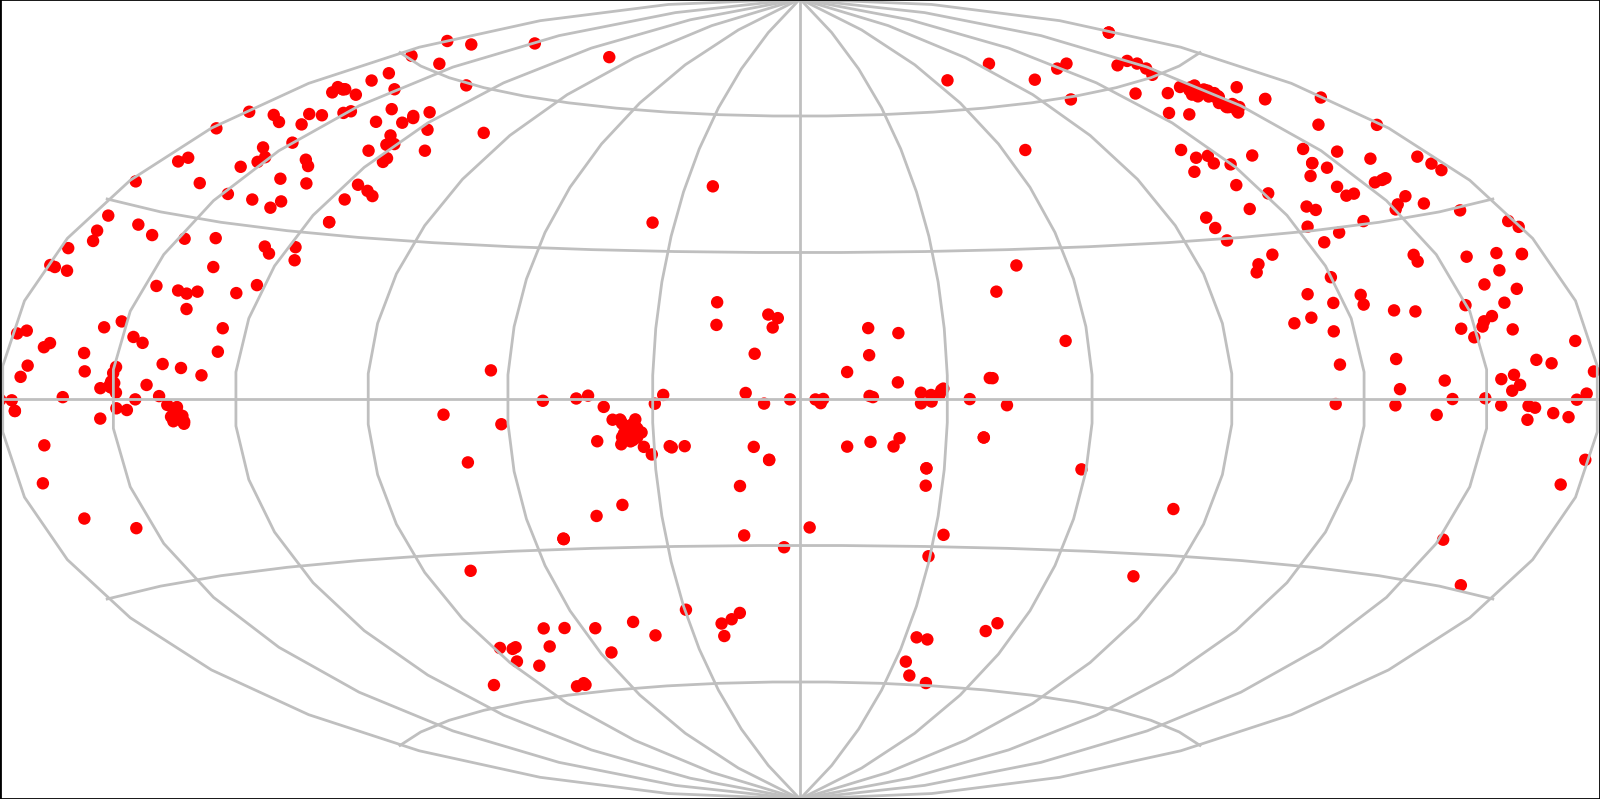
\includegraphics[width=\hsize]{fig/lenssky}
\caption{Sky distribution of 423 published lenses considered secure
  (from the Masterlens catalog at the University of Utah, maintained
  by Joel Brownstein and Leonidas Moustakas).  The map is in
  Hammer-Aitoff projection, with North up and $\rm RA=0$ in the
  middle. The empty swathes to the left and right of centre are the
  Milky Way. {\em Should we drop this figure?  It's not relevant to
    modelling, but as there seems to be no publicly available summary
    of all known lenses, it does help set context.}}
\label{fig:masterlens}
\end{figure}

Surveys now under way aim to increase the inventory of lenses another
ten or a hundred fold.  Among these is \sw (Marshall et al, in prep,
More et al, in prep).  \sw is a citizen science project\footnote{\tt
  http://www.spacewarps.org} in which volunteers are presented
sky-survey images and invited to identify lens candidates.  Simulated
lenses are mixed in with the data, both to help train volunteers on
what to look for, and to provide measures of the effectiveness of the
search.  The motivation for \sw is to enable volunteers, some of whom
had previously serendipitously identified lens candidates on earlier
citizen-science surveys, to make discoveries missed in automatic
searches by software robots.  Robots are very good with clean lensing
system in uncrowded fields with high signal-to-noise, but in general
test situations \citep{2009ApJ...694..924M} robots miss lenses (low
completeness) or contaminate the results with non-lenses (low purity).
\sw introduced its first tranche of survey data, in May 2013.  The
Canada-France-Hawaii Telescope Legacy Survey (CFHTLS), covering
$\simeq172$ square degrees (0.4\% of the sky) was divided into tiles
of $80''\times80''$ ($440\times 440$ pixels).  Each such tile was
shown to ten volunteers.  Despite the rarity of detectable lenses
($<10^{-3}$ per tile), the \sw collective soon found lens candidates,
both rediscoveries already known from robots \citep{Gavazzi2012,
  More2012ApJ} and possible new lenses.

The encouraging early results prompted the question: could modeling of
the lenses also be done by volunteers?  An early proposal for what
became \sw included a prototype lens modelling tool
\citep{2010AAS...21543527N}.  There are several software tools for
lensing modelling available, and work has been done on generic
interfaces \citep{2013NewAR..57....1L,2014A&C.....5...28L}.  Moreover,
some {\em Spacewarps\/} volunteers are quite experienced from earlier
projects, having spent a thousand hours or more with data, and very
interested in more demanding projects.  The interests of
citizen-science communities are just beginning to be studied
\citep[e.g.,][]{2013AEdRv..12a0106J}, but it is clear that some
volunteers welcome open-ended challenges, and sometimes these have led
to new scientific results: one example is the discovery of an
exceptional extra-solar planet \citep{2013ApJ...768..127S}; another is
the development of new algorithms for protein folding
\citep{Khatib22112011}.  All these are grounds for optimism.  There
is, however, a basic difficulty in strong gravitational lensing.
Lensed images do not look much like their source, and still less do
they resemble the lensing-mass distribution.  To model a lens, one
needs to either do a lot of random guessing, or have a good intuition
for what works.

In this paper, we propose a way around the difficulty, and report on a
modelling test on \sw using simulated lenses.  There are three aspects
to this work, covered in the following three sections.

In section \secref{Fermat} we introduces a theoretical innovation,
which we call a ``spaghetti diagram''.  This is a cartoon-like markup
of a lensed system, which implicitly encodes the basis of a mass
model.  A spaghetti diagram is basically the saddle-point contours
originally introduced to gravitational lensing by
\cite{1986ApJ...310..568B} as a way of classifying lensed images.
They are sometimes shown as part of the output of lens models
\citep[for
  example][]{2001ApJ...557..594R,2003ApJ...590...39K,Lubini2012}.  In
the present work, however, spaghetti diagrams are the {\em input\/}
through which the modeller tells the program what to do.

In section \secref{SpaghettiLens} we describe the \spl program, which
implements everything.  \spl is an extension of the GLASS framework
for modelling lenses \citep{2014arXiv1401.7990C}.  \spl is designed to
be friendly to the forum style of citizen-science projects, without
sacrificing any features of GLASS.  The program is invoked online, and
the modelling history is logged in a transparent way, enabling forum
discussions and incremental improvement by different people.
Moreover, any result can be revisited and post-processed if desired.
These features are of general interest for citizen-science projects,
but somewhat outside the scope of the present paper.


The purpose of this study was to provide a means to model a large number of gravitational lenses by showing that gravitational lens modeling can be learned / done by volunteers.
We suggest, that volunteers will be as successful as professionals with modeling if provided with an easy to use tool with visual feedback (What you see is what you get, WYSIWYG) and a minimal set of instructions.
Volunteers will then crowd work (using buzz word here ;) ) / work collaborative on modeling lenses from several sources / groups at a central place.
Since this is an iterative learning process, the more involved volunteers will quickly gain knowledge that can be passed down to new volunteers.
That creates a social structure that scales well with the number of volunteers, as other projects have already shown. %TODO \needcite
Finding people working as volunteers has been shown to be successful last but not least by \sw and the whole galaxy zoo project.
To test the people's abilities, we investigated the performance of a few volunteers modeling a set of simulated lenses.
We tested the ability to correctly identify lensed images and reproduce similar mass map of the lens.

It is well known that making a scientific contribution is a central
motivation cited by citizen-science volunteers.  So for a lens
modeler in a citizen-science project, nobody wants that it should
sacrifice scientific usefulness in order to be fun to use.  That said,
being aesthetically pleasing and having a short initial learning curve
are also essential qualities.  Also desirable is that the user is
encouraged/challenged to go deeper and wider into the subject.
  \spl tries to address all of these.

\section{Fermat's principle and spaghetti diagrams} \label{sec:Fermat}

We now explain spaghetti diagrams and then outline what \spl does with
them.

\subsection{Geometrical and gravitational time delays} 

Let us recall the formulation of gravitational lensing by
\cite{1986ApJ...310..568B} in terms of Fermat's principle .  Consider
a lens at some redshift $z_L$ and let $(x,y)$ be planar coordinates at
the lens, transverse to the line of sight.  Let $\Sigma(x,y)$ be the
mass per unit area, projecting along the line of sight.  This surface
density is often given in a dimensional form
\begin{equation} \label{eq:kappa}
\kappa(x,y) \propto \Sigma(x,y) \,.
\end{equation}
Consider also a more distant light source, at redshift $z_S$, behind
point $(x_s,y_s)$ on the lens.

Now imagine a virtual photon coming from the source to some $(x,y)$ on
the lens, then changing direction and coming to the observer.  Such a
direction change would increase the light travel time compared to
coming through $(x_s,y_s)$.  The increased light travel time from the
geometry of deflection would be
\begin{equation} \label{eq:tgeom}
\tgeom(x,y) \propto (x-x_s)^2 + (y-s_y)^2 \,.
\end{equation}
assuming it is small compared to the total light travel time.

An additional delay of the photon comes from travelling through the
curved spacetime at the lens, and can be related to the mass
distribution of the lens by an implicit relation, as follows.  The
value of $\tgrav$ through $(x,y)$ equals its average value on the
circumference of a small circle centred at $(x,y)$, plus a constant
times the mass within that circle.  The proportionality constant is
$2G/c^3$ times the cosmological expansion factor $(1+z_L)$. Thus
\begin{equation} \label{eq:tgrav}
\tgrav(x,y) = \left\langle \tgrav(x_\subcirc,y_\subcirc) \right\rangle
              + (1+z_L) \frac{2G}{c^3} M(x_\subbullet,y_\subbullet) \,.
\end{equation}
We have used $(x_\subcirc,y_\subcirc)$ to denote the circumference of
a circle, and $(x_\subbullet,y_\subbullet)$ to indicate the integrated
mass within the circle.

The light travel time of a virtual photon is therefore longer by
\begin{equation}  \label{eq:tarriv}
t(x,y) = t_{\rm geom} + t_{\rm grav} \,.
\end{equation}
than it would have been with no lens present.  Real photons take paths
that make $t(x,y)$ extremal, that is, having a minimum, maximum or
saddle point (Fermat's principle).

The proportionality factors in \eqref{eq:kappa} and \eqref{eq:tgeom}
depend on the redshifts and cosmological parameters and are given in
the Appendix~\ref{more-theory}.

\begin{figure}
\centering
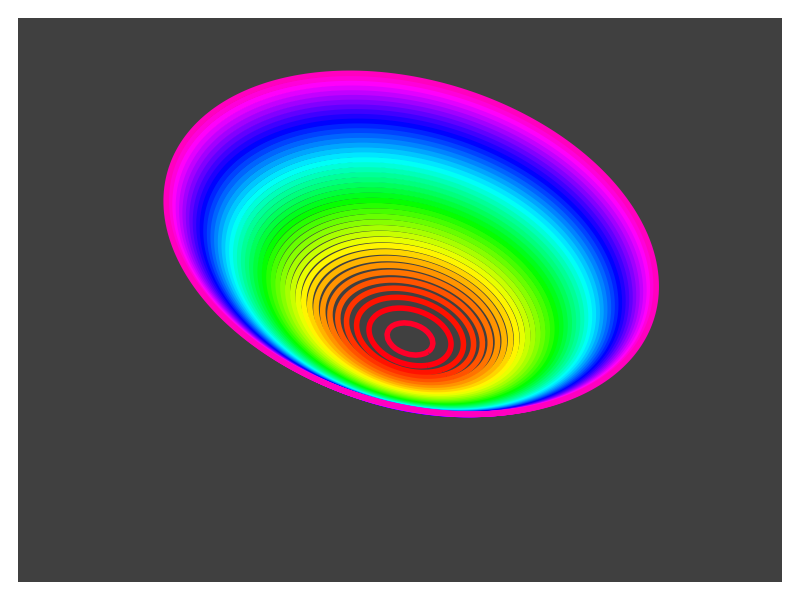
\includegraphics[width=\columnwidth]{fig/arriv_0}
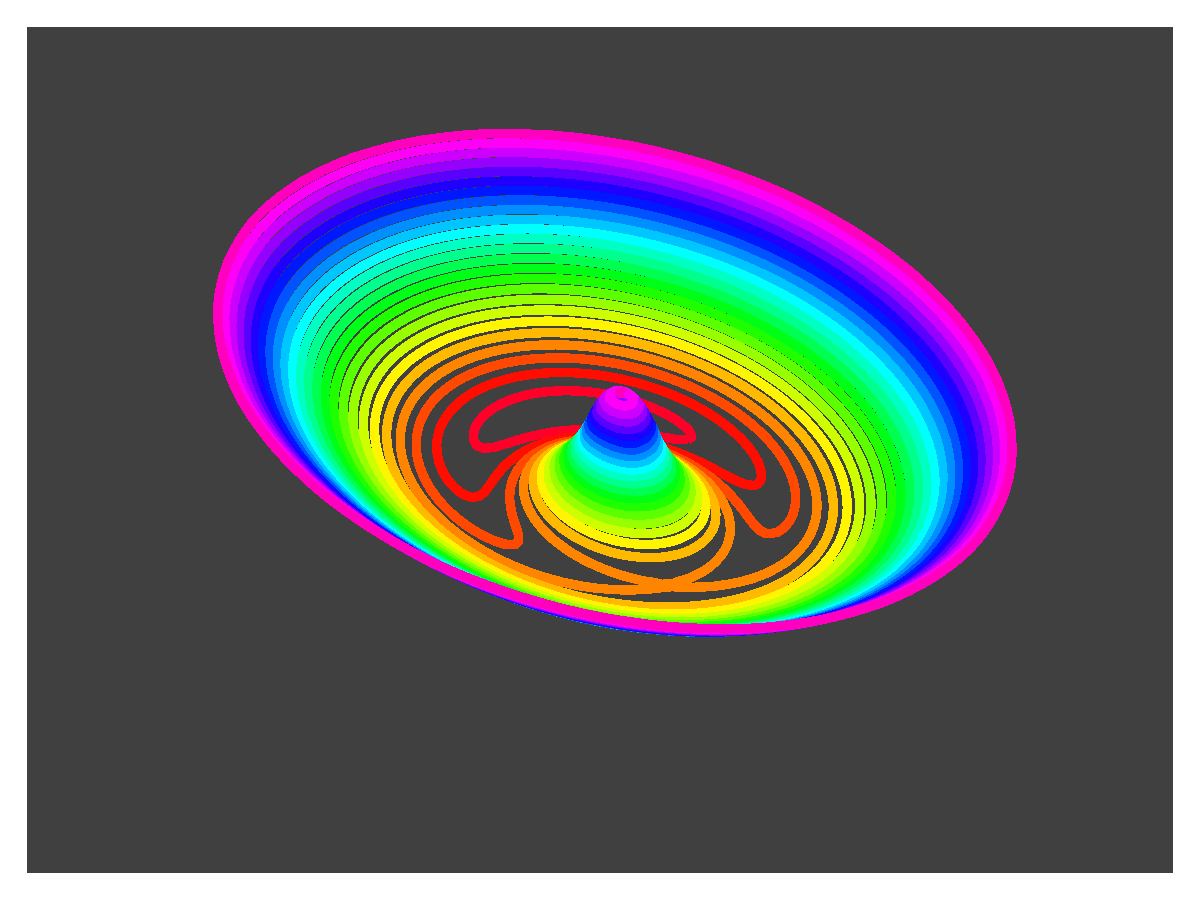
\includegraphics[width=\columnwidth]{fig/arriv_1}
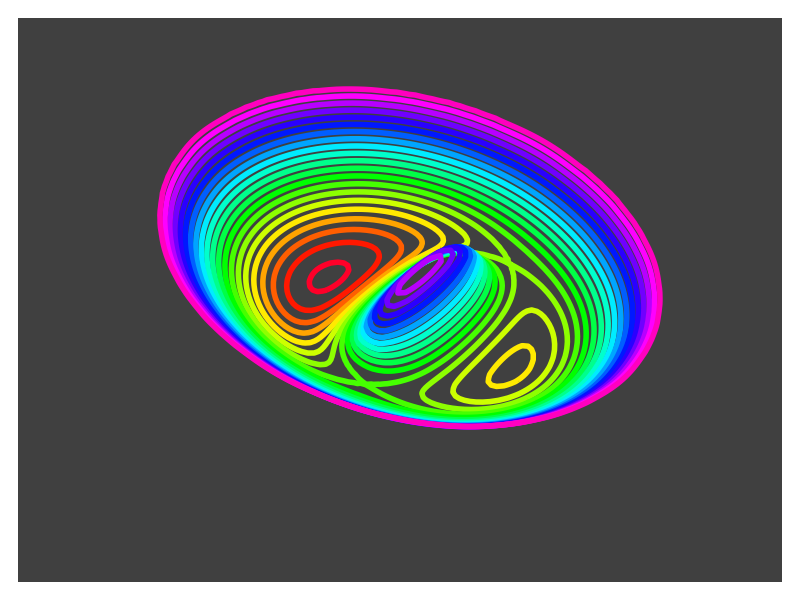
\includegraphics[width=\columnwidth]{fig/arriv_2}
\caption{Perspective views and contour maps of example arrival time
  surfaces.  Contours are coloured in rainbow order (red: least delay,
  violet: highest delay).  {\em Upper panel:\/} No lens, hence showing
  the parabolic shape of the geometrical time delay.  The image would
  be at the bottom, coinciding with the source. {\em Middle panel:\/}
  A circular lensing mass (offset from the source) has been added,
  which has pushed the minimum to one side and introduced a maximum
  and saddle point, each corresponding to an image.  The saddle-point
  is characterized by a self-crossing ``spaghetti'' contour. {\em
    Lower panel:\/} An elongated lensing mass has been added.  There
  are now two minima, two saddle points, and a maximum, each
  corresponding to an image.  Note the two self-crossing spaghetti
  contours associated with the saddle points.}
\label{fig:arriv}
\end{figure}


\subsection{Arrival-time contours} \label{sec:arriv}

The full function $t(x,y)$, also known as the arrival-time surface,
applies to virtual photons.  In other words, it is an abstract
construct and not itself observable.  But observable image positions
can be derived from the arrival-time surface, so visualising it is
useful.  Figure~\figref{arriv} does so.  In this figure, a maximum,
where present, is easy to see.  To locate mimima and saddle-points,
however, one needs to examine the contours of equal arrival time.  A
saddle point is characterised by a contour crossing itself, forming
an~X.  Mimima, on the other hand, have contours looping around them,
as do maxima.

The saddle-point contours which form an X are especially interesting,
because they set the overall topography of the arrival-time surface.
The obviously give the locations of the saddle points, and roughly
localise the minima and maxima as well.  If more precise locations of
the minima and maxima are added, the whole arrival-time surface is
already approximately known.  Since the arrival-time surface has an
exact relation to the lens-mass distribution and the source position,
in effect the mass distribution is also automatically specified.  In
other words, a simple sketch of saddle-point contours along with
locations of minima and maxima ---which we call a spaghetti diagram---
is implicitly already an approximation to a lens-mass distribution.
This idea is the basis of \spl.

The preceding assumes a point source.  To get an idea of what an
extended source would do, let us imagine moving the original source
slightly.  The contours of constant arrival time will naturally move
slightly, and so will the images.  The movement of the contours will
be most noticeable where the contours are far apart, that is where the
arrival-time surface is nearly flat.  As is evident from
\figref{arriv}, this is the region where the minimum and saddle points
lie, or near the images.  In this region, points on the source that
are close together produce images that are comparatively far apart.
In other words, the image is highly magnified.  In summary, lower
curvature in the arrival-time surface for a point source implies
larger magnification of an extended source.  Conversely, where the
arrival-time surface is strongly curved, the image will be
demagnified.  We see from \figref{arriv} that the arrival-time surface
tends to be highly curved near the maximum.  Hence maximum tend to be
demagnified.  In practice, maxima of the arrival time are nearly
always too faint to see. The minima and saddle points dominate.

\section{A lens-modelling program} \label{sec:SpaghettiLens}

\spl implements the ideas of the arrival-time surface into a modeling
program.

The first modeling step with \spl is for the user to call up the \sw
of interest, and make an educated guess for the topography of the
arrival-time surface --- specifically, the locations of the maxima,
minima and saddle points that correspond to images of the brightest
part of the source.  Input is given by tracing a proposal for the
saddle-point contours.  \Figref{input-spag} shows some example
inputs --- and incidentally also indicates the origin of the name
\spl.

\spl, as implemented so far, assumes that the lens is dominated by a
single galaxy, and that the center of that galaxy is the sole maximum.
Once the maximum has been identified, we wish to characterize the rest
of the arrival-time surface in relation to it.  From geometry, any
surface that has a central maximum and goes high at the edges must
have a lima\c con-like contour, meaning a two-looped curve with one
loop inside the other.  The maximum lies within the inner loop, a
minimum lies between the two loops, and a saddle point lies at the
self-intersection of the contour.  The top panel of
\figref{input-spag} shows an example: red marks a suggested
maximum, green a saddle point, and blue a minimum.  (The small pink
dots are just help sketch the proposed contour.)  The middle and lower
panels of \figref{input-spag} show a more complex situation.
The minimum has split into three images: two new minima with a saddle
point in between.  In this situation the contour through the new
saddle point forms a figure of eight, its two loops enclosing the two
new minima.  The configuration of a lima\c con, possibly with a figure
of eight inside, suffices to give a preliminary description of the
arrival-time surface for nearly all cases where the lens is dominated
by one galaxy, and the source is a single small object.

The exact placement of the pink spaghetti loops shown in
\Figref{input-spag} has no significance.  Their utility is
just to help mark up the image as maximum, minima and saddle points.
As the figure suggests, the marking up can be done very easily with a
mouse.  Human intuition is required to (a)~identify lensed images and
separate them from other background light sources, and (b)~classify
and order images according to arrival time.  But the computer helps by
allowing only valid lensing configurations to be entered, and ensuring
that the odd image theorem is taken care of.%TODO \needcite

In the second modeling step, once the user has sketched a proposed
spaghetti configuration, \spl sends the input to its server-side
modeling engine, called GLASS \citep{2014arXiv1401.7990C}.  The task
of GLASS is to find a mass distribution $\kappa(x,y)$ that exactly
reproduces the locations of the maximum, minima and saddle
points. Now, this criterion by itself is extremely under-determined
--- there are infinitely many mass distributions that will reproduce a
given set of maxima, minima and saddle points, but typically they
(a)~produce lots of extra images, and (b)~look very unlike galaxies.
Additional assumptions (a prior) are necessary.  GLASS uses a prior
based on suggestions by \cite{1997MNRAS.292..148S}.
\begin{enumerate}
\item The mass distribution is built out of non-negative tiles of
  mass.  (Sometimes these tiles are called mass pixels, but we should
  emphasize that they are unrelated to image pixels, and are much
  larger.)
\item There is a notional lens center, say $(x_0,y_0)$ which is
  identified with the maximum of the arrival time.  The source can
  have an arbitrary offset with respect to the lens center.
\item The mass distribution must be centrally concentrated, in two
  respects.  First, the circularly averaged density must fall away
  like $$ \left[(x-x_0)^2+(y-y_0)^2\right]^{-1/2}$$ or more steeply.
  Second, the direction of increasing density at any $(x,y)$ can point
  at most $45^\circ$ away from $(x_0,y_0)$.
\item The lens must be symmetrical with respect to $180^\circ$ rotations
  about $(x_0,y_0)$.  This symmetry assumption can be relaxed if the
  user wishes.
\end{enumerate}
There are still infinitely many models that satisfy both data and
prior constraints, but now they are more credible as galaxy lenses.
It is then possible to generate an ensemble of models.  The sampling
technique used by GLASS is described in \citep{Lubini2012}, and
improves upon earlier techniques \citep{2000AJ....119..439W,Saha2004}.
Typically, ensembles of 200 models are used.  That is to say, what we
call a \spl model is really the mean of an ensemble of 200 models, and
its estimated uncertainty is the range covered by the whole ensemble.

In the third modeling step, having generated a model ensemble, \spl
post-processes it to present results and diagnostics to the user for
inspection. This takes the form of three figures.
\begin{enumerate}
\item A synthetic image of the lensed features.
\item A contour map of the arrival-time surface.
\item A gray scale plus contour map of the mass distribution.
\end{enumerate}
After examining this feedback, the user can archive the results for
discussion, or modify their input and try again, or discard the
attempt altogether.

The fourth modeling step is discussion among modelers and iteration on
the model.  Any archived model can be revised by another user: they
can modify the spaghetti configuration slightly or drastically, or
change options like the size of the mass tiles.  Particularly
interesting lens candidates lead to trees of models in this way.
Forum discussion then prunes the tree, focusing attention on one or a
few models.\footnote{See ``Collaborative gravitational lens
  modelling\dots'' in {\tt http://letters.zooniverse.org} for an
  example.}


\section{A lens modeling challenge} \label{sec:mod_challenge}

Interested volunteers from the \sw forum were initially introduced to
\spl through a video tutorial and by videocon.  After this
introductory stage, a modeling challenge was presented.  This
consisted of 29 simulated lenses (sims) covering a range of lensing
configurations.

The \sw sims were generated by AM, in consultation with PM and AV.
To estimate the performance of the volunteers and the quality of the generated models, two analysis  were done.
The first analysis tested the correct identification and ordering of lensed images.
The second one compared the mass distribution of the lens $\kappa(x, y)$ of the generated models to the mass distribution of the simulations.

A challenge set of 29 was selected, representing the different image
morphologies among the spacewarps sims.  Modellers then contributed
129 models for these sims (at least for each sim).  Models were
collecting in the same forum used to model real candidate lenses, and
under the same conditions --- modellers were free to consult and
refine each other's models, but had no information on how the sims
were generated.

\subsection{The simulated lenses} \label{sec:sims}

The sims were produced using {\tt gravlens}
\citep{2001astro.ph..2341K,2001astro.ph..2340K} using the CFHTLS survey data
and catalogues \cite{Coupon2009}. They were of three
kinds, as follows.

\begin{enumerate}
  \item Imitating lensed quasars: having a singular elliptical
    isothermal lens (SIE) plus constant external shear, and a circular
    Gaussian source.
  \item Emulating lensed galaxies: similar to the above, but with an
    elliptical de Vaucouleurs source.
  \item Resembling cluster lenses: having a source as above, but a
    more complicated lens, with one dominant elliptical SIE and
    one or more perturbing elliptical SIEs, plus a circular NFW
    \citep{1996ApJ...462..563N,1997ApJ...490..493N} to represent
    the underlying dark matter distribution.
\end{enumerate}

Formulas for the lenses appear in \cite{2001astro.ph..2341K}. The SIE
lenses follow equations (33--35) of that work, with core radius set to
zero.  The NFW lens is in equations (48) and (50), while shear is the
$\gamma$ term in equation (76).

The information in this section was not revealed to the person
choosing the challenge set (RK) or to the modellers (EB, CC, CM, PS,
JO and JW) until the modeling stage was done.

\subsection{Some example models} \label{sec:example_models}

The modellers proposed a total of 129 models for the 29 sims in the
challenge. Typically XX models were produced per simulation, with XX
systems having only XX models (corresponding tot he most simplest
simulations) to XX having XX models (a complex and contrversial lens
system). In the following we discuss eight example lenses in detail
with individual notes per system and corresponding plots are shown in
figures 4-11 (or whatever compact version you end up making). These
eight examples were chosen on the basis of …??

The modelers proposed a total of 129 models for the 29 sims in the
challenge.  Figures \ref{fig:6941} to \ref{fig:6919} show eight of
models in some detail.

\FloatBarrier

\begin{figure}
  \centering
  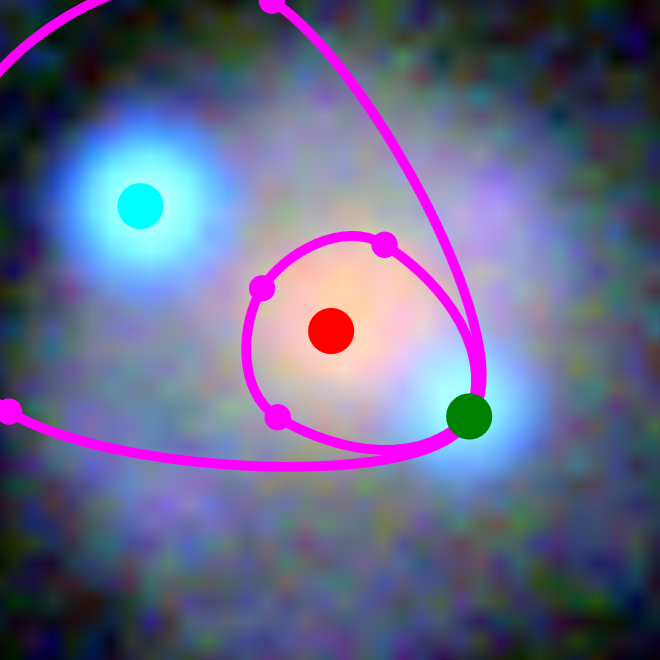
\includegraphics[width=\myplotswidth]{fig/006941_input}
  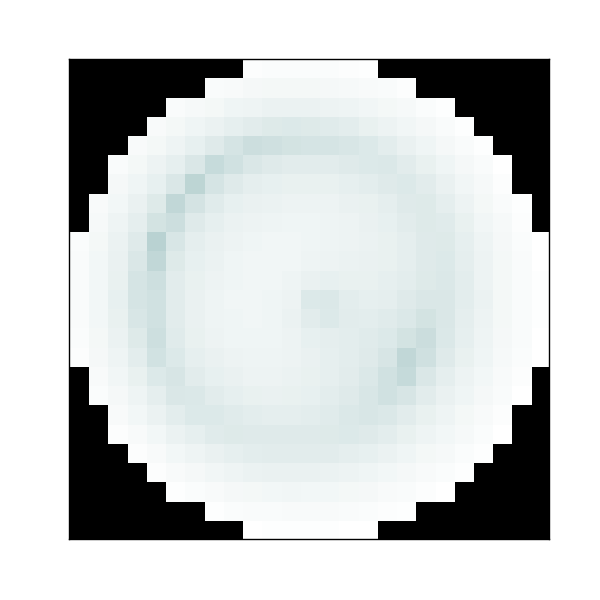
\includegraphics[width=\myplotswidth]{fig/006941_arr_time} \\
  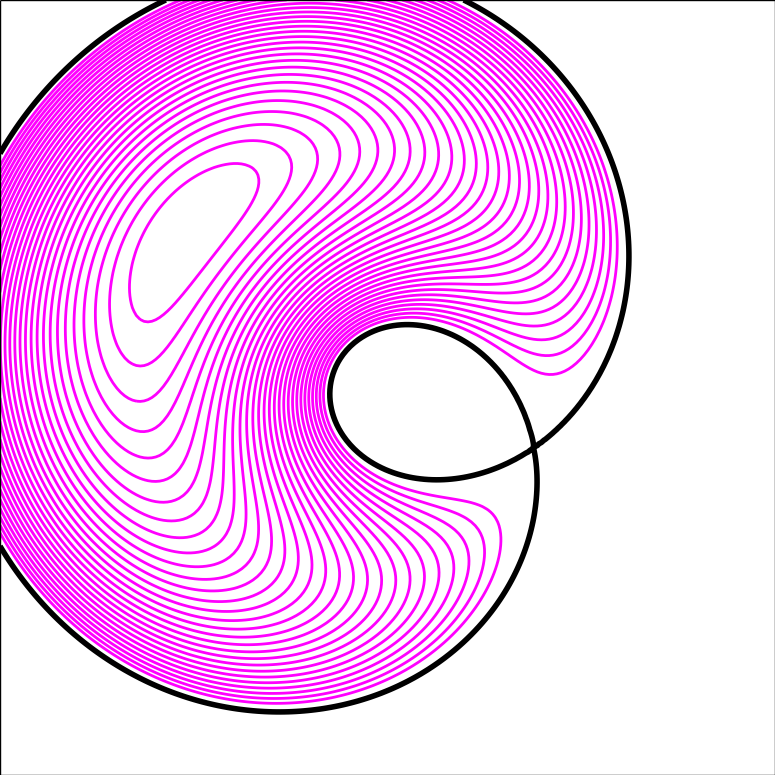
\includegraphics[width=\myplotswidth]{fig/ASW000102p_006941_arriv} 
  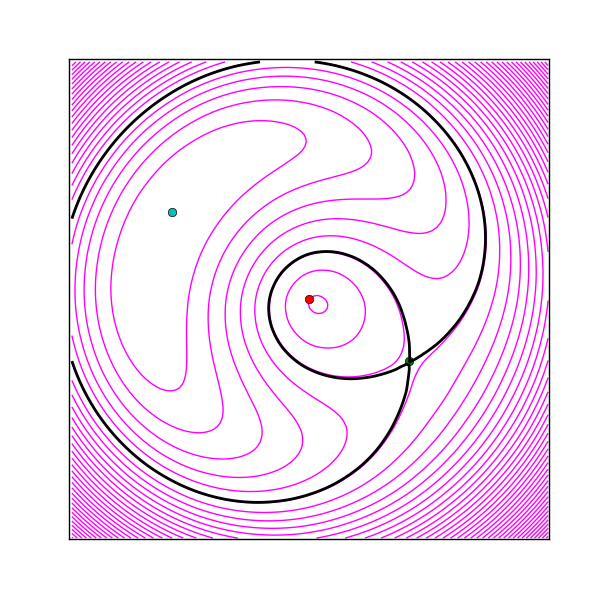
\includegraphics[width=\myplotswidth]{fig/006941_spaghetti} \\
  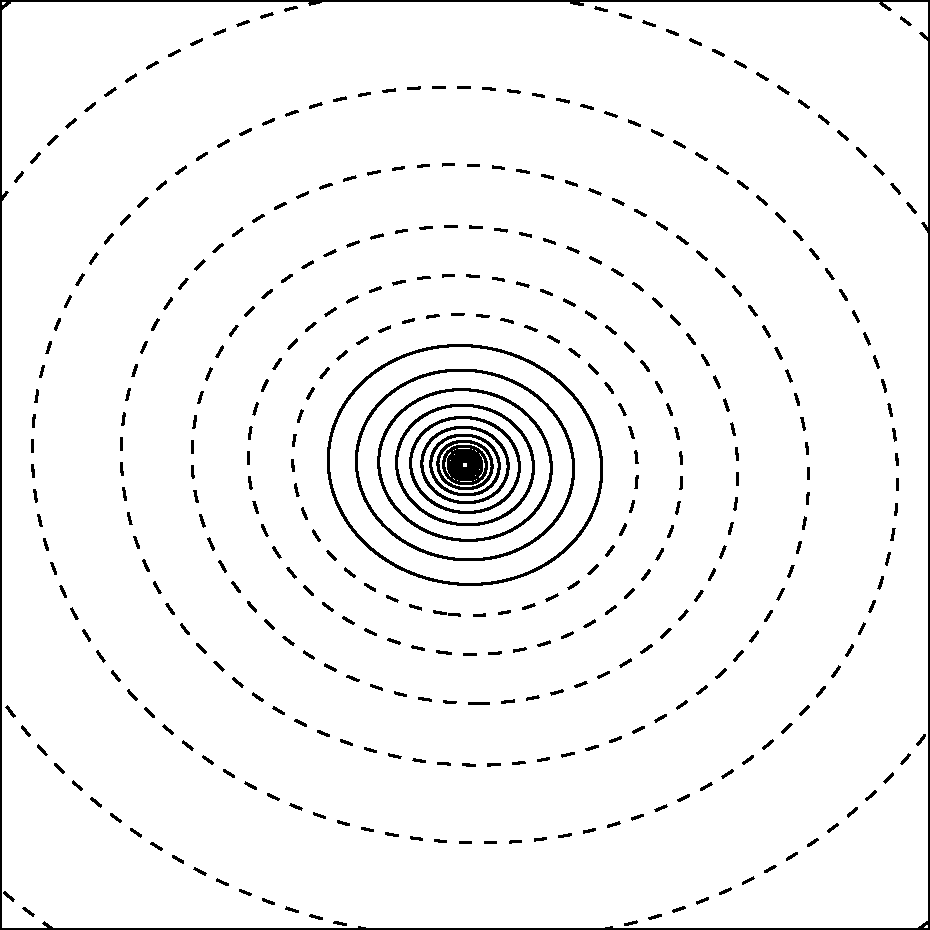
\includegraphics[width=\myplotswidth]{fig/ASW000102p_006941_kappa}
  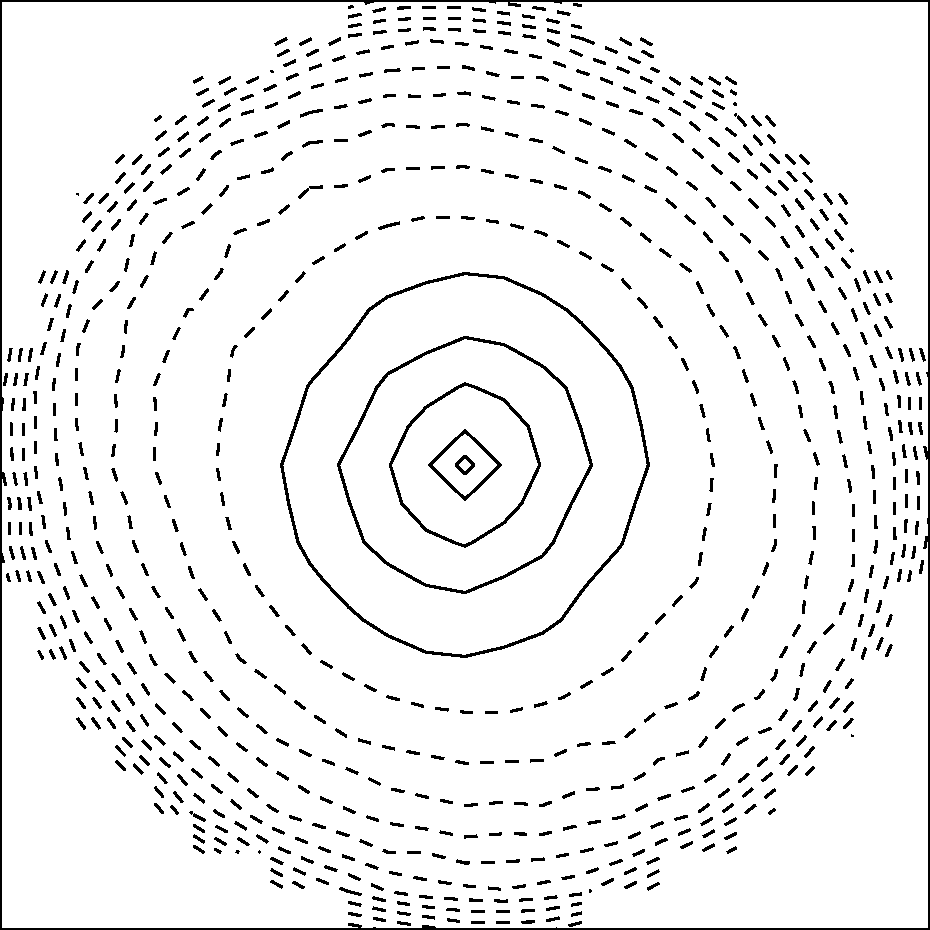
\includegraphics[width=\myplotswidth]{fig/006941_mass}
  \caption[result 6941 (ASW000102p)]{A simulated lens that mimics a
    lensed quasar, and model results.  The left panels derive from the
    simulation, and the right panels are \spl output.  Details of
    individual panels are in \ref{sec:example_models}.}

  \label{fig:6941}
\end{figure}

\begin{figure}
  \centering

  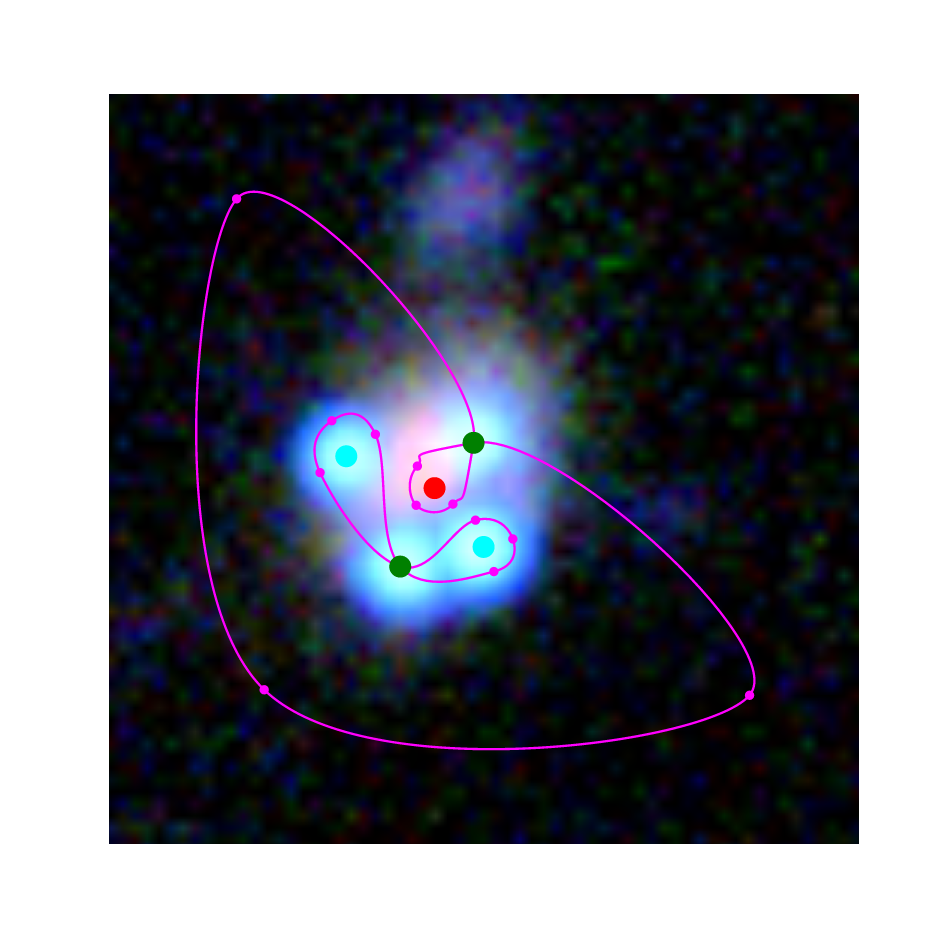
\includegraphics[width=\myplotswidth]{fig/006915_input}
  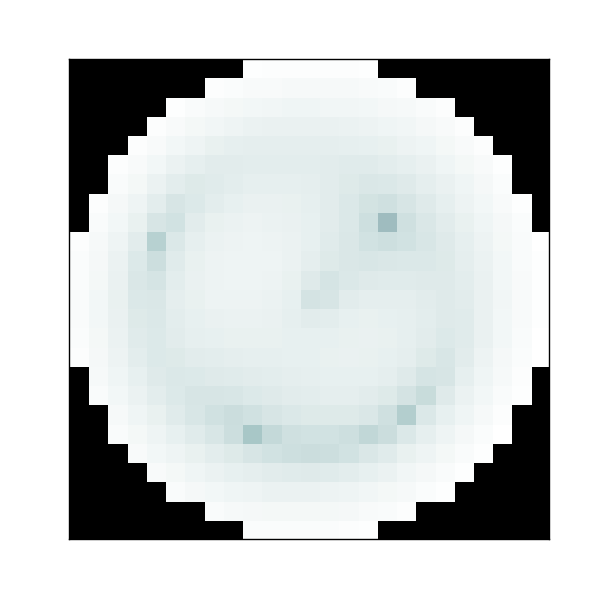
\includegraphics[width=\myplotswidth]{fig/006915_arr_time} \\
  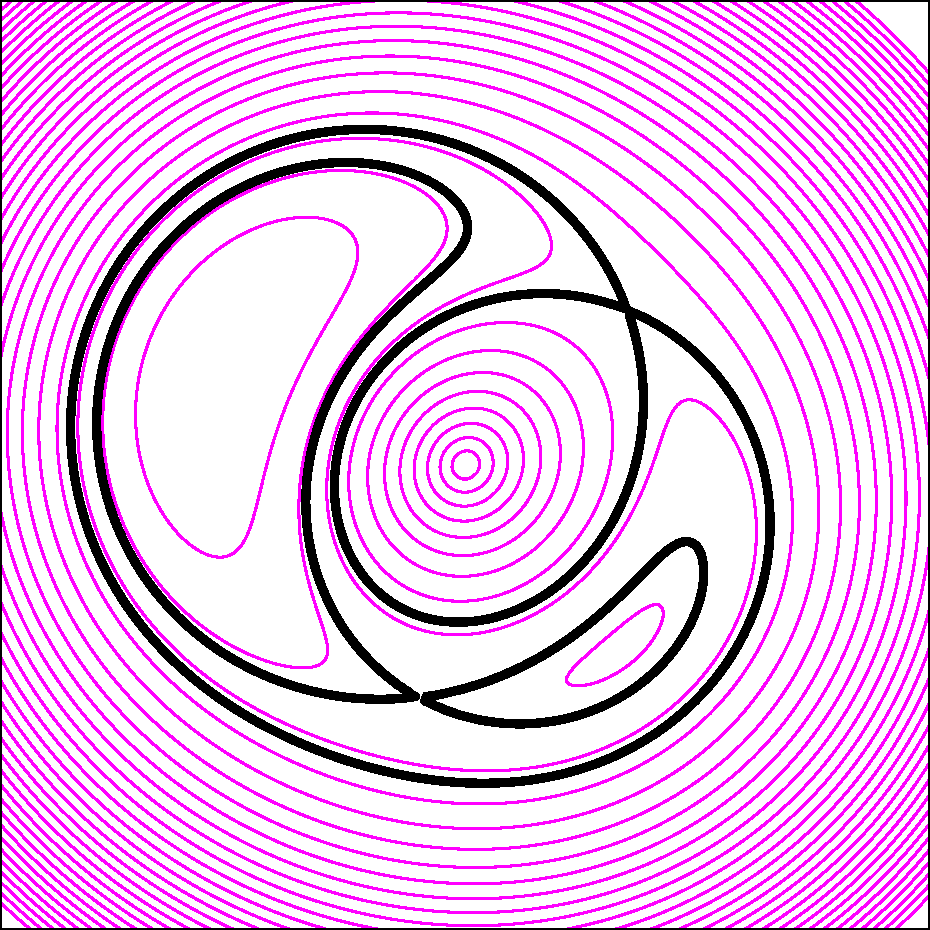
\includegraphics[width=\myplotswidth]{fig/ASW0001hpf_006915_arriv}
  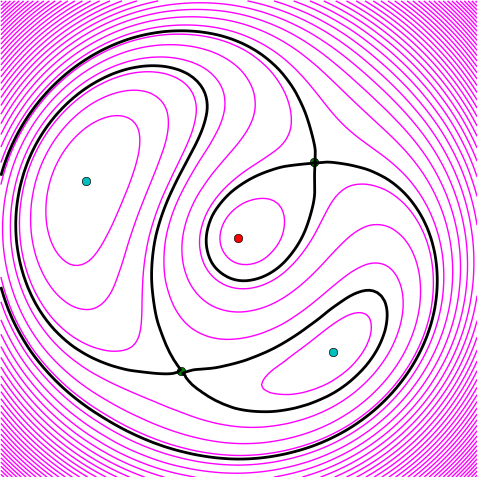
\includegraphics[width=\myplotswidth]{fig/006915_spaghetti} \\
  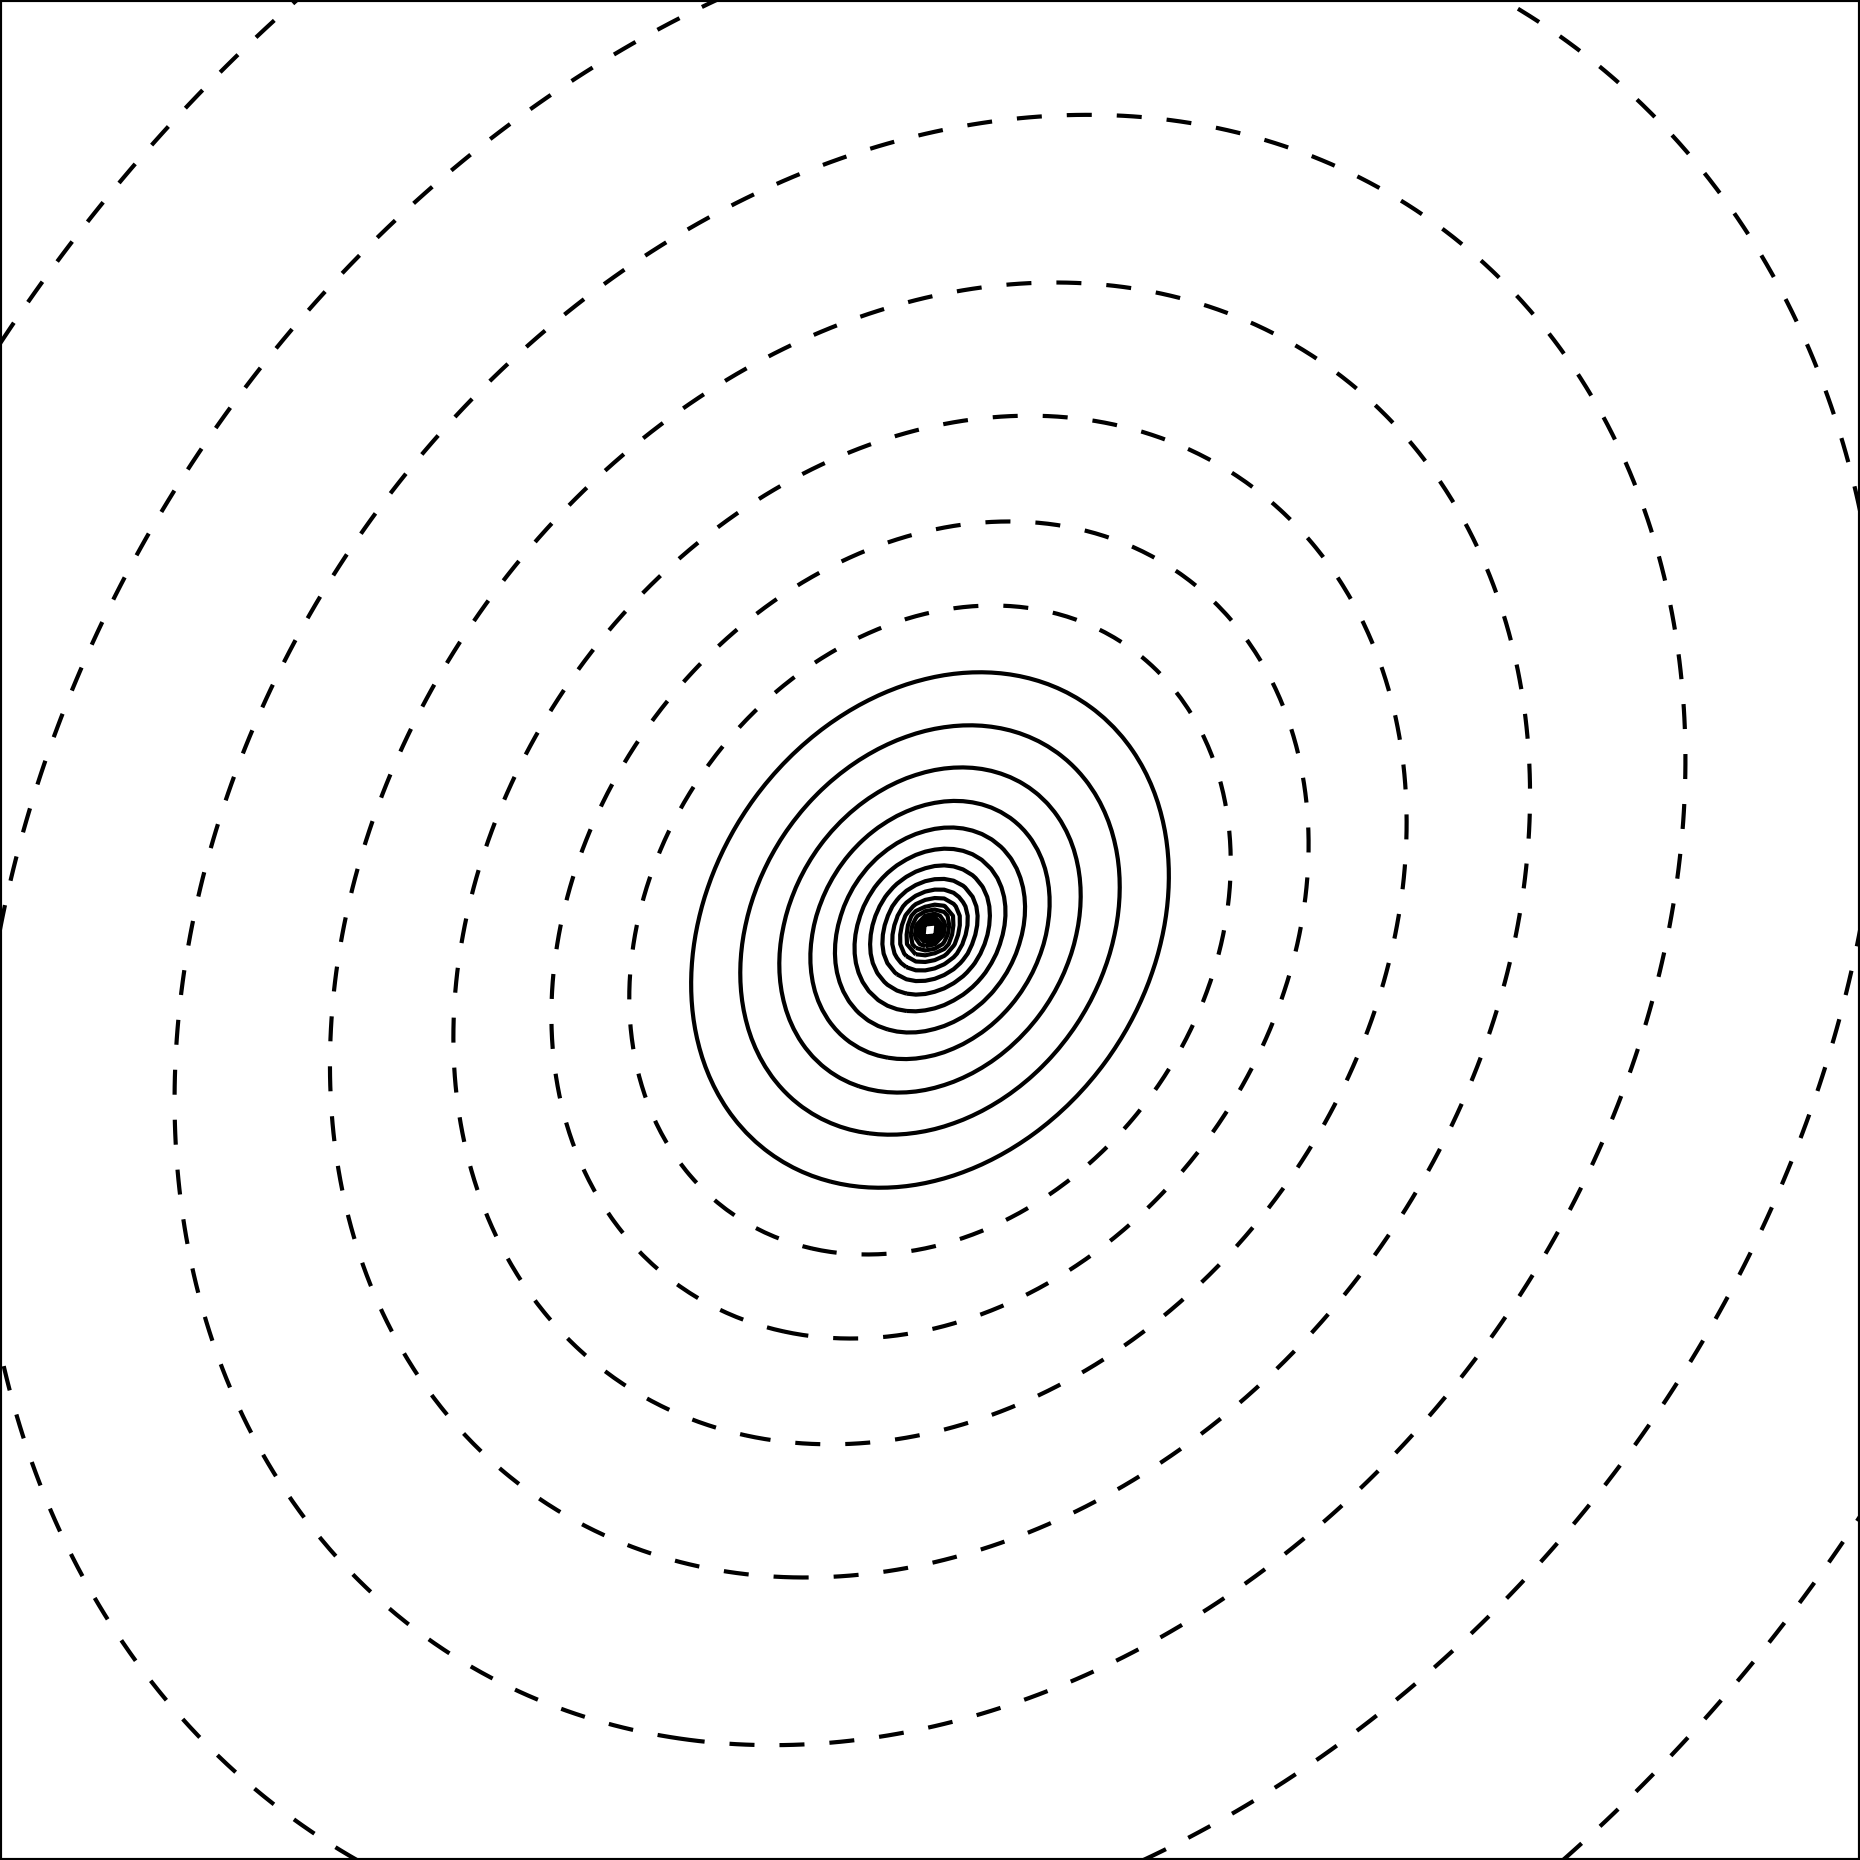
\includegraphics[width=\myplotswidth]{fig/ASW0001hpf_006915_kappa}
  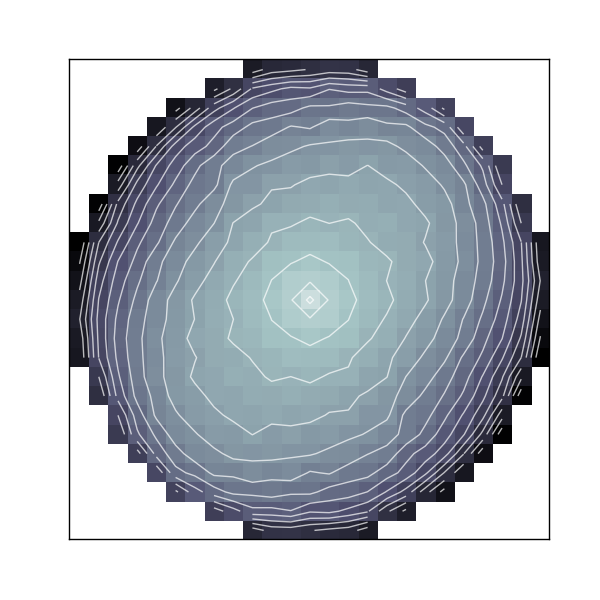
\includegraphics[width=\myplotswidth]{fig/006915_mass}

  \caption[result 6915 (ASW0001hpf)]{A four-image configuration
    typical of lensed quasars. (See Section \ref{sec:example_models}
    for details.)}
  \label{fig:6915}
\end{figure}


\begin{figure}
  \centering
  
  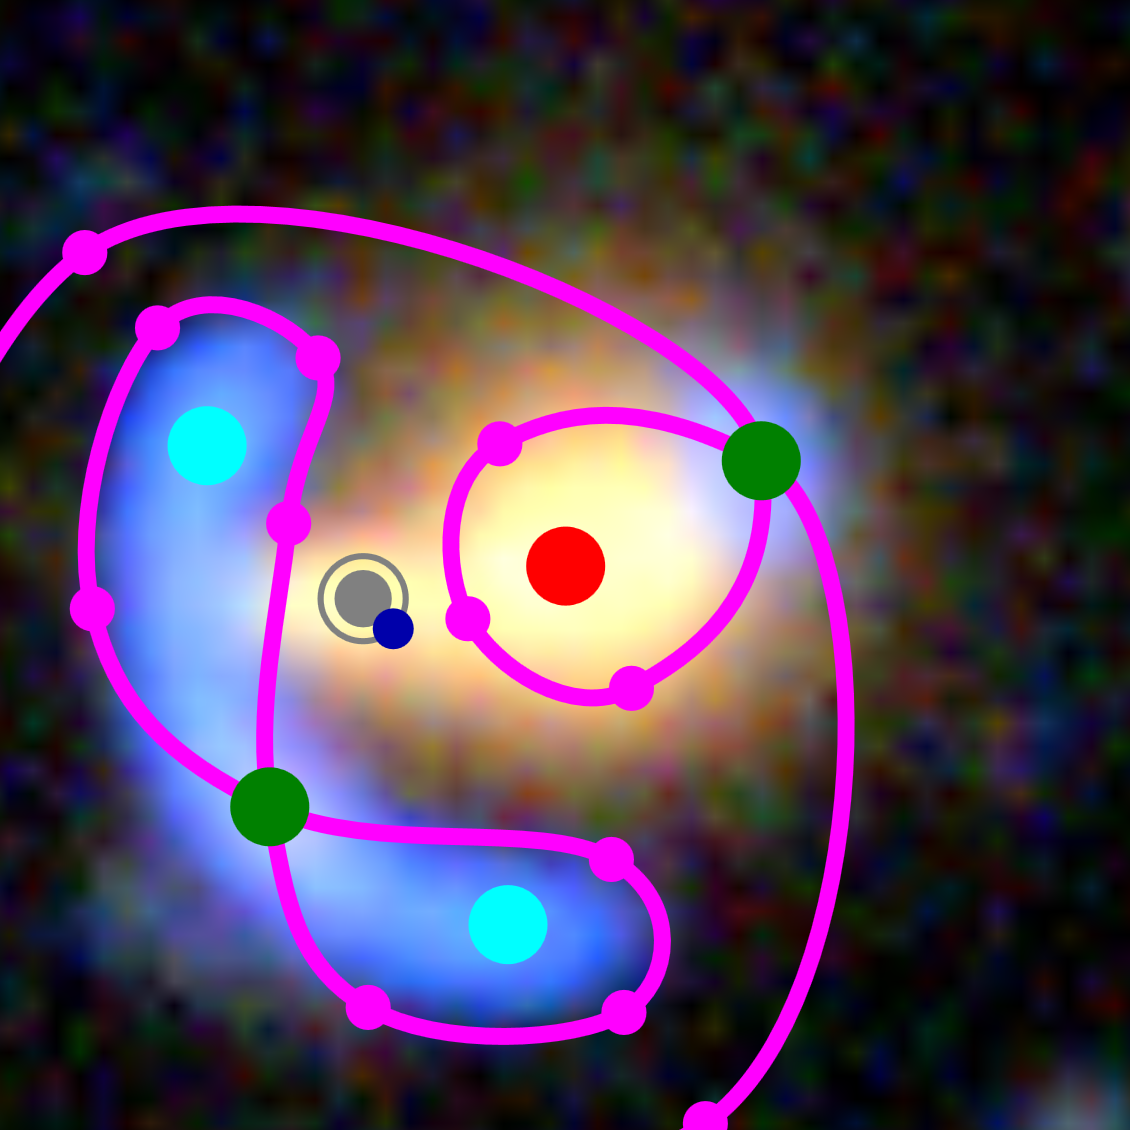
\includegraphics[width=\myplotswidth]{fig/006990_input}
  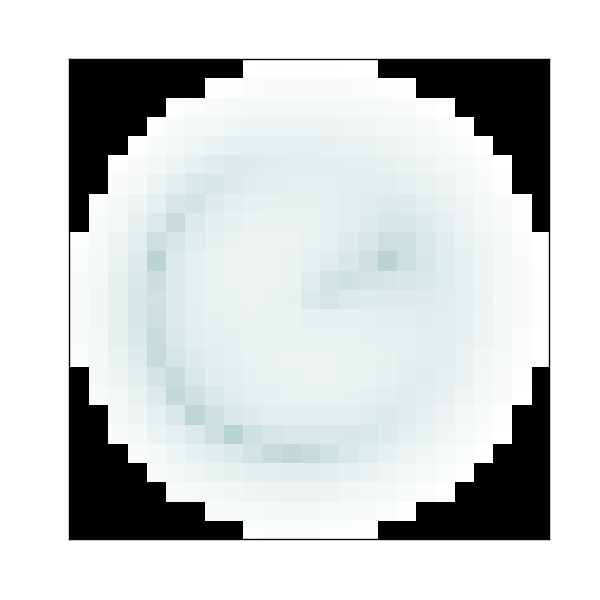
\includegraphics[width=\myplotswidth]{fig/006990_arr_time} \\
  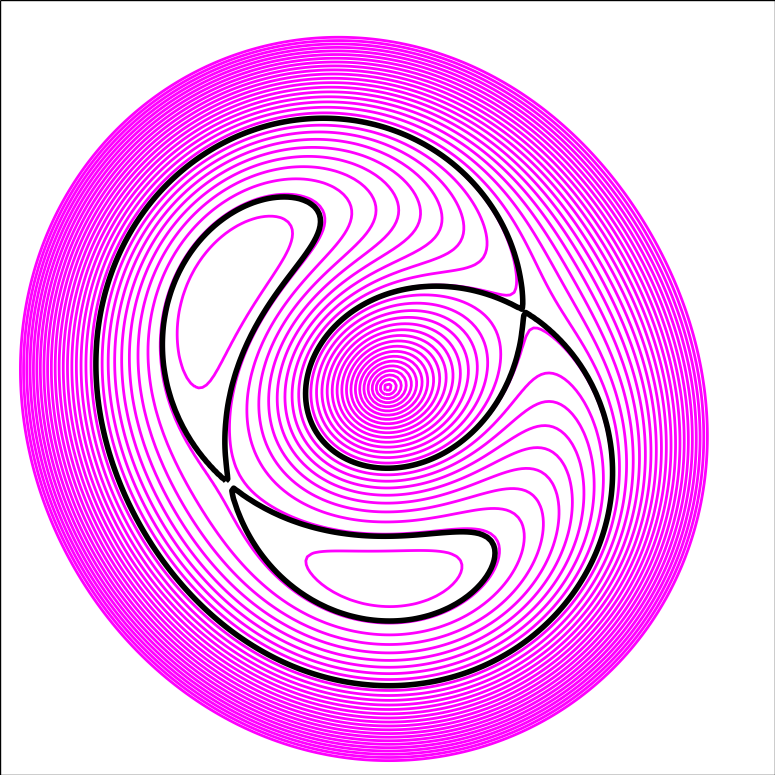
\includegraphics[width=\myplotswidth]{fig/ASW0004oux_006990_arriv}
  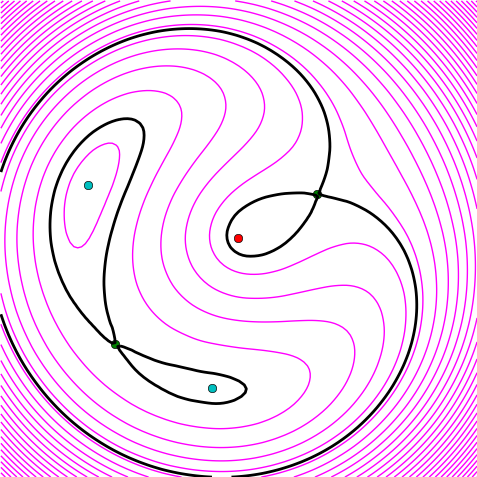
\includegraphics[width=\myplotswidth]{fig/006990_spaghetti} \\
  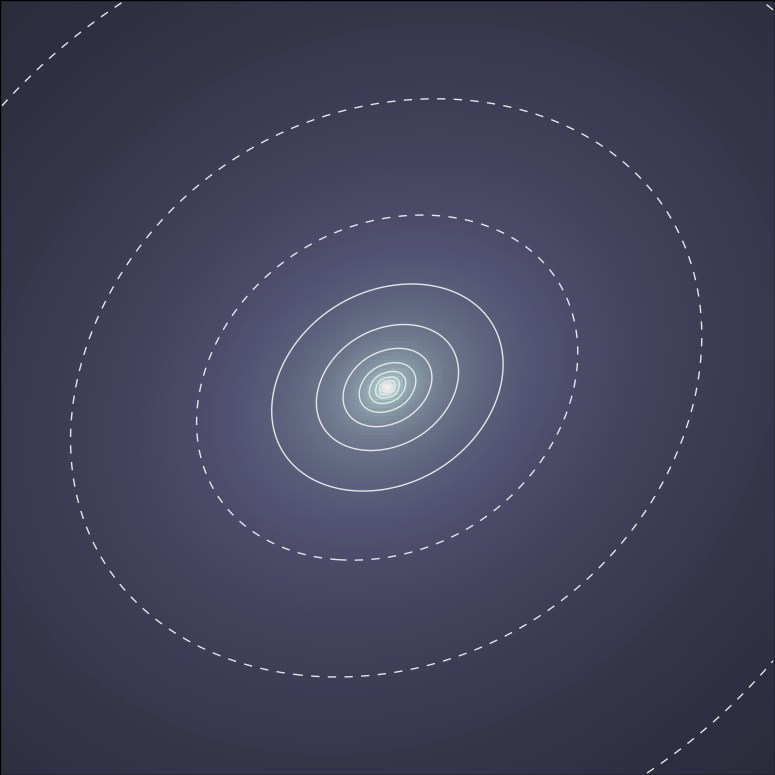
\includegraphics[width=\myplotswidth]{fig/ASW0004oux_006990_kappa}
  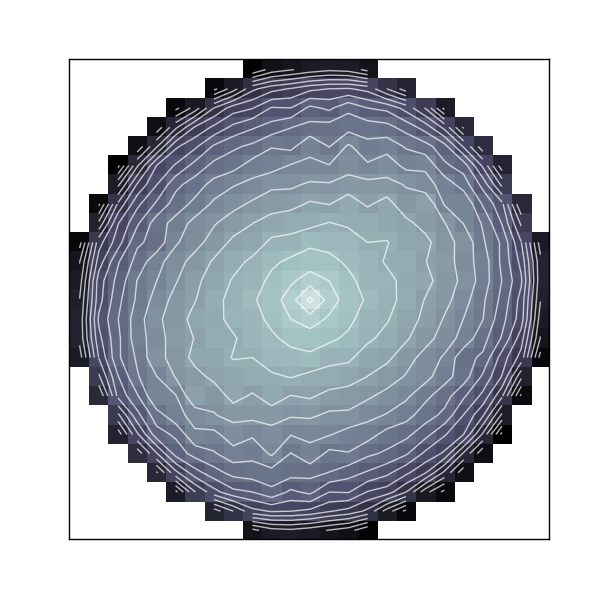
\includegraphics[width=\myplotswidth]{fig/006990_mass}

  \caption[result 6990 (ASW0004oux)]{Results from a system with an arc
    plus a counter-image, typical of lensed galaxies. (See Section
    \ref{sec:example_models} for details.)}
  \label{fig:6990}
\end{figure}



\begin{figure}
  \centering

  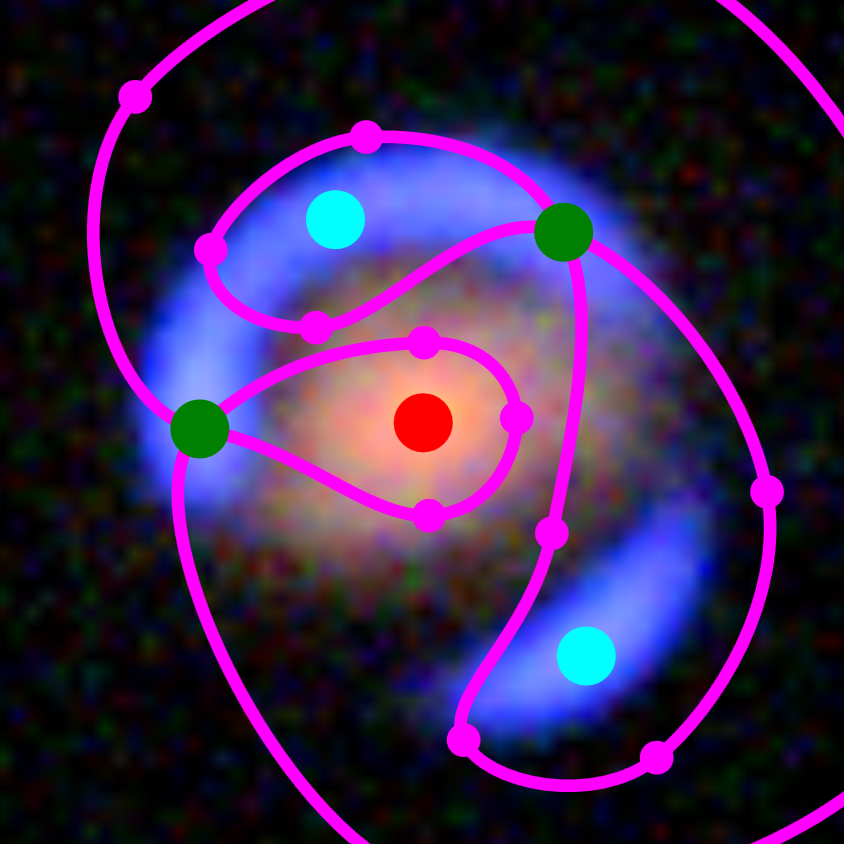
\includegraphics[width=\myplotswidth]{fig/006919_input}
  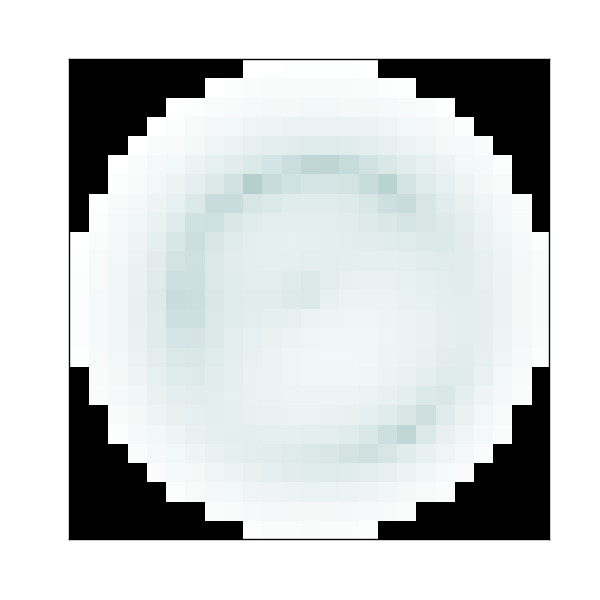
\includegraphics[width=\myplotswidth]{fig/006919_arr_time} \\
  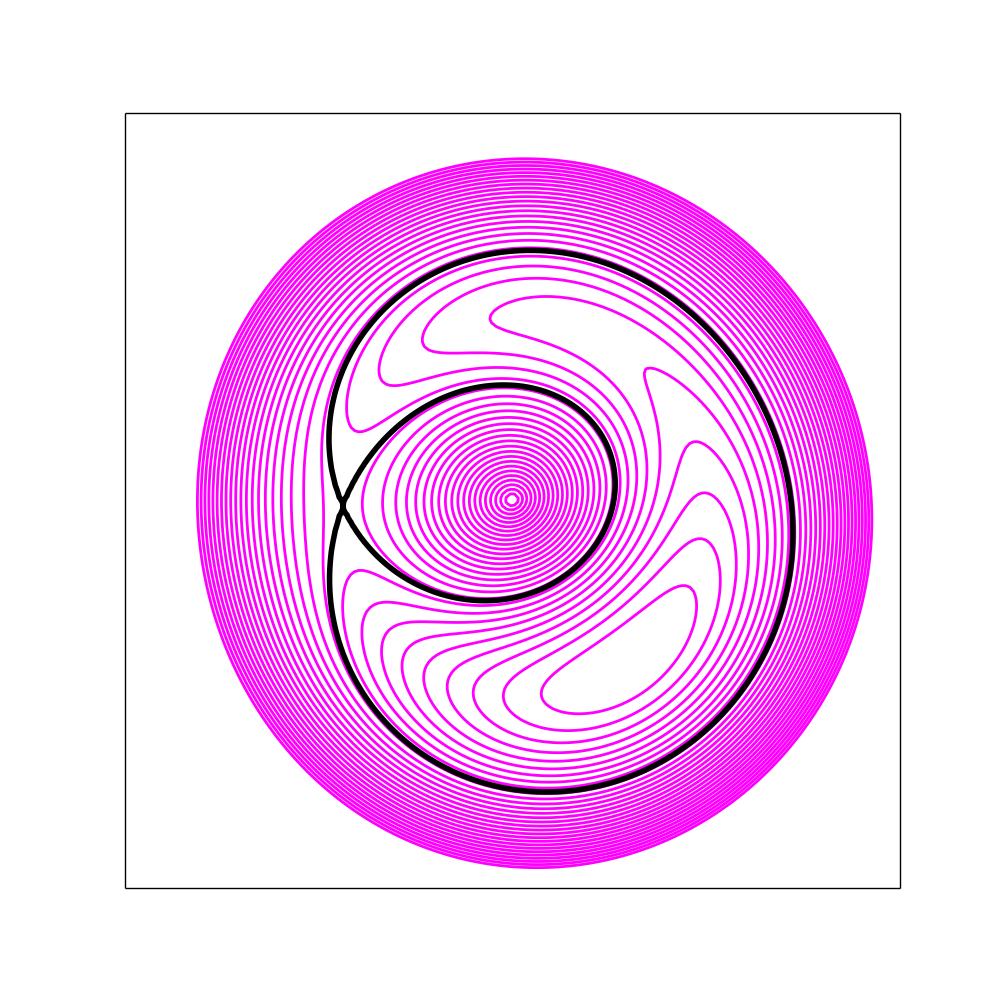
\includegraphics[width=\myplotswidth]{fig/ASW0002z6f_006919_arriv}
  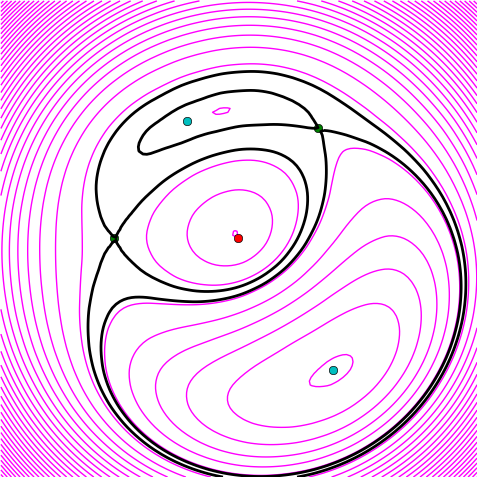
\includegraphics[width=\myplotswidth]{fig/006919_spaghetti} \\
  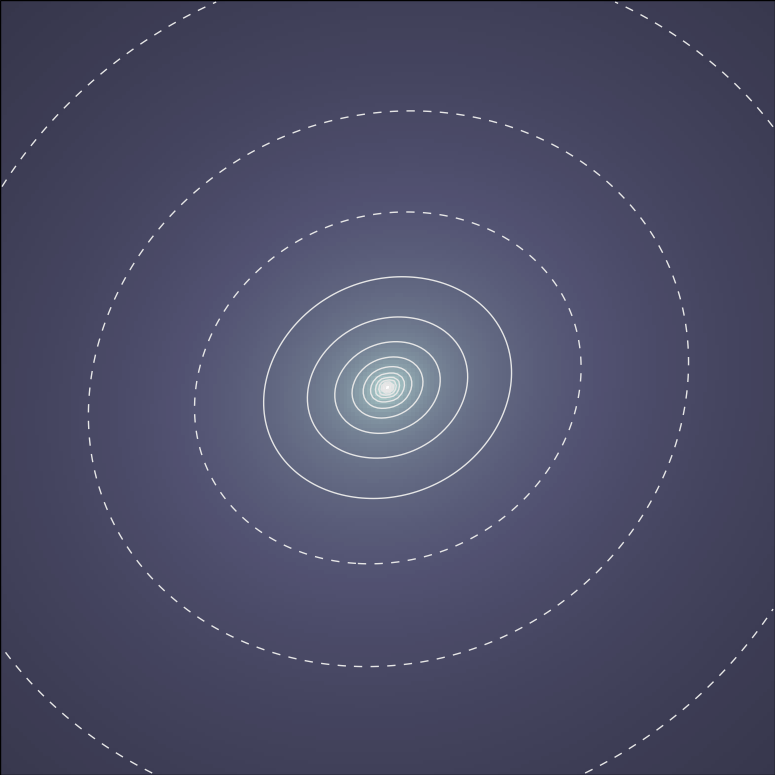
\includegraphics[width=\myplotswidth]{fig/ASW0002z6f_006919_kappa}
  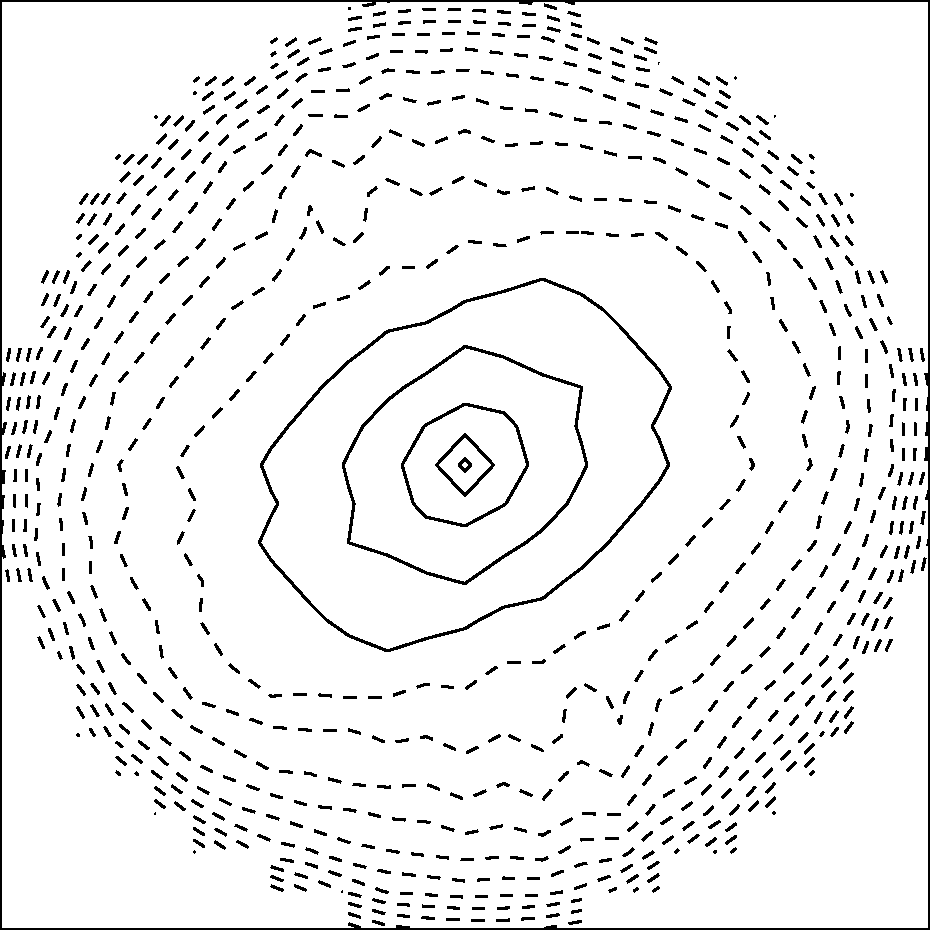
\includegraphics[width=\myplotswidth]{fig/006919_mass}

  \caption[result 6919 (ASW0002z6f)]{Another configuration of arc plus
    counter-image; here the arc is closer to the lensing galaxy than
    the counter-image. (See Section \ref{sec:example_models} for
    details.)}
  \label{fig:6919}
\end{figure}



\begin{figure}
  \centering
  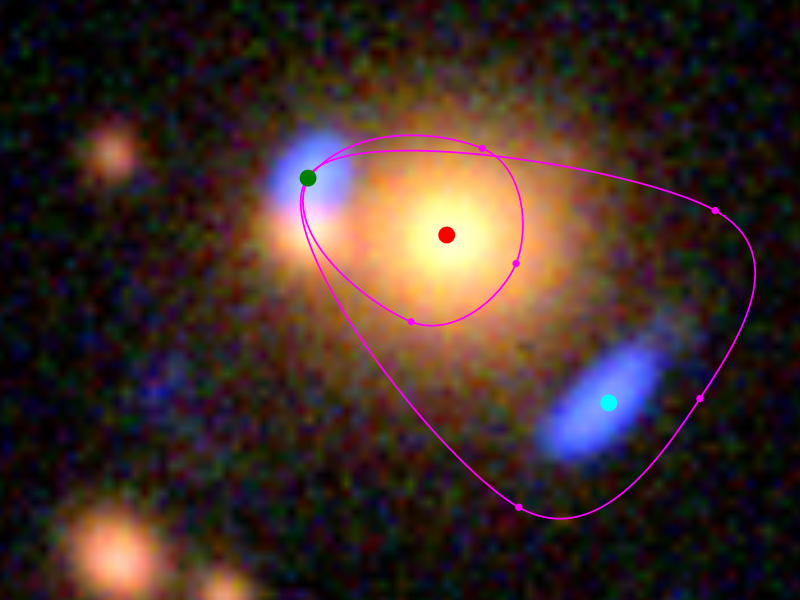
\includegraphics[width=\myplotswidth]{fig/006975_input}
  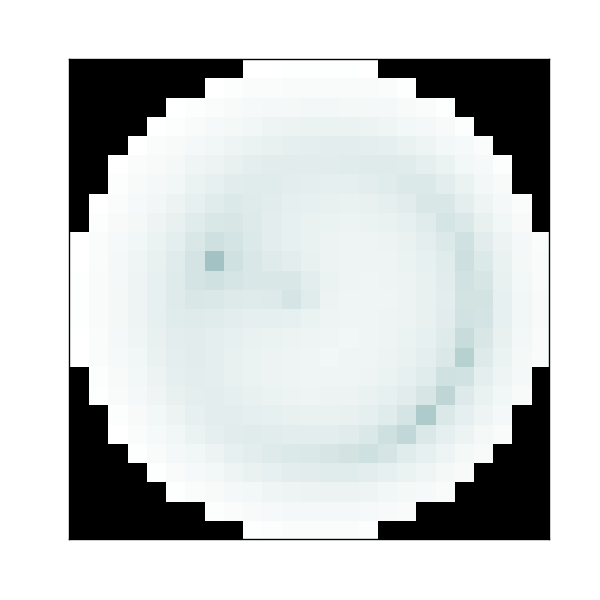
\includegraphics[width=\myplotswidth]{fig/006975_arr_time} \\
  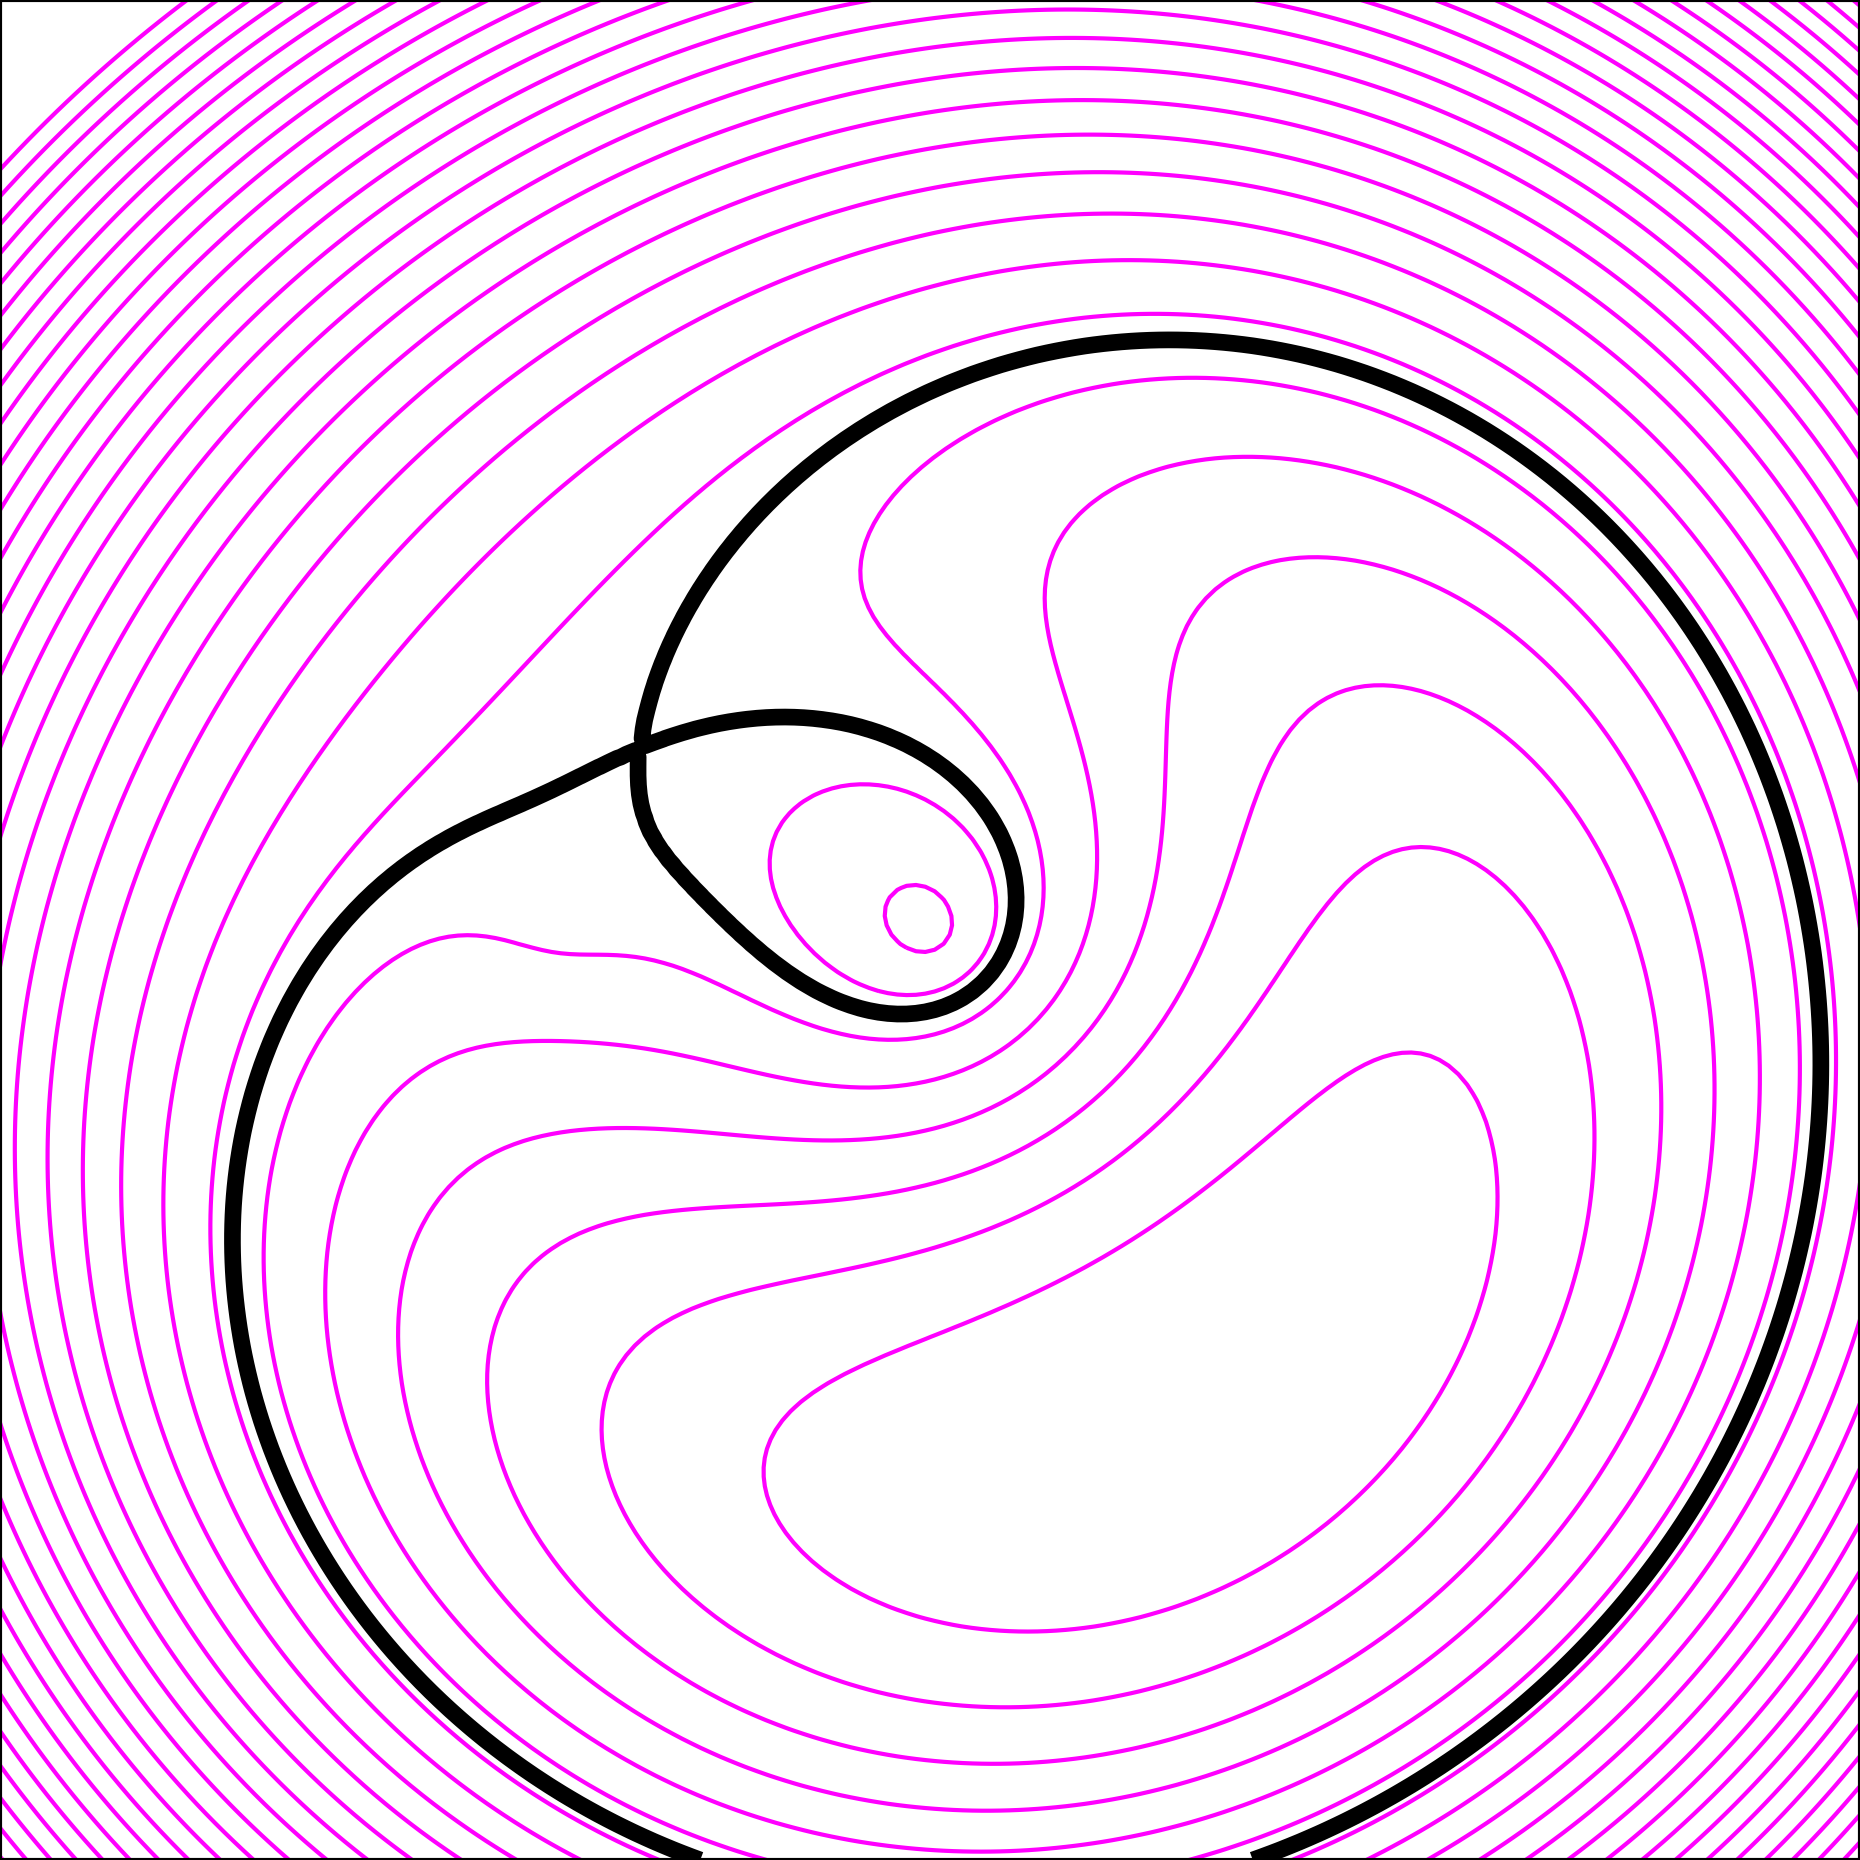
\includegraphics[width=\myplotswidth]{fig/ASW000195x_006975_arriv.png}
  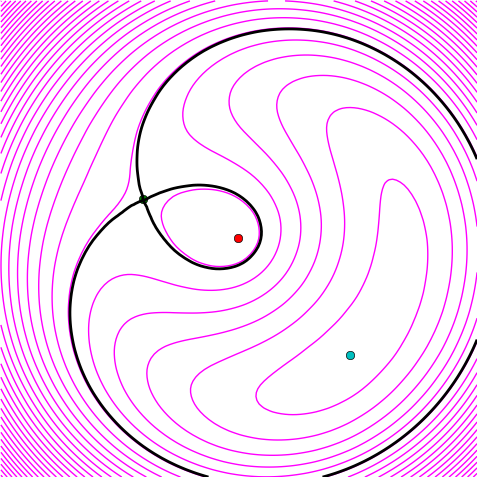
\includegraphics[width=\myplotswidth]{fig/006975_spaghetti} \\
  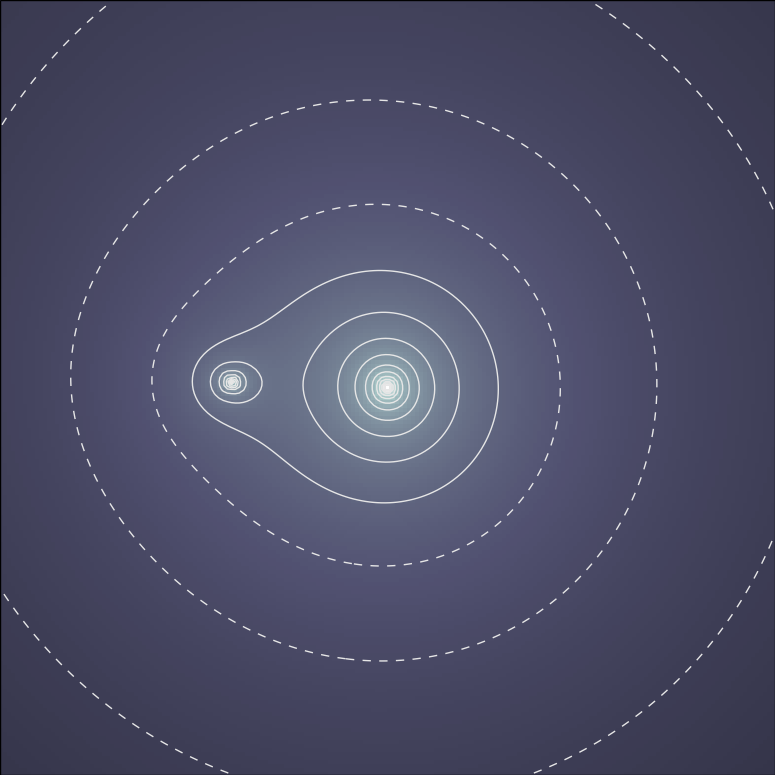
\includegraphics[width=\myplotswidth]{fig/ASW000195x_006975_kappa.png}
  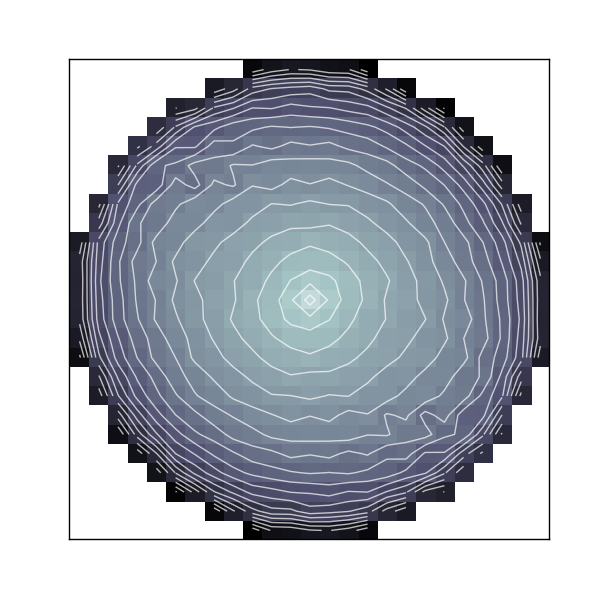
\includegraphics[width=\myplotswidth]{fig/006975_mass}
  \caption[result 6975 (ASW000195x)]{A lens with unrecovered mass
    substructure. (See Section \ref{sec:example_models} for details.)}
  \label{fig:6975}
\end{figure}
  
\begin{figure}
  \centering

  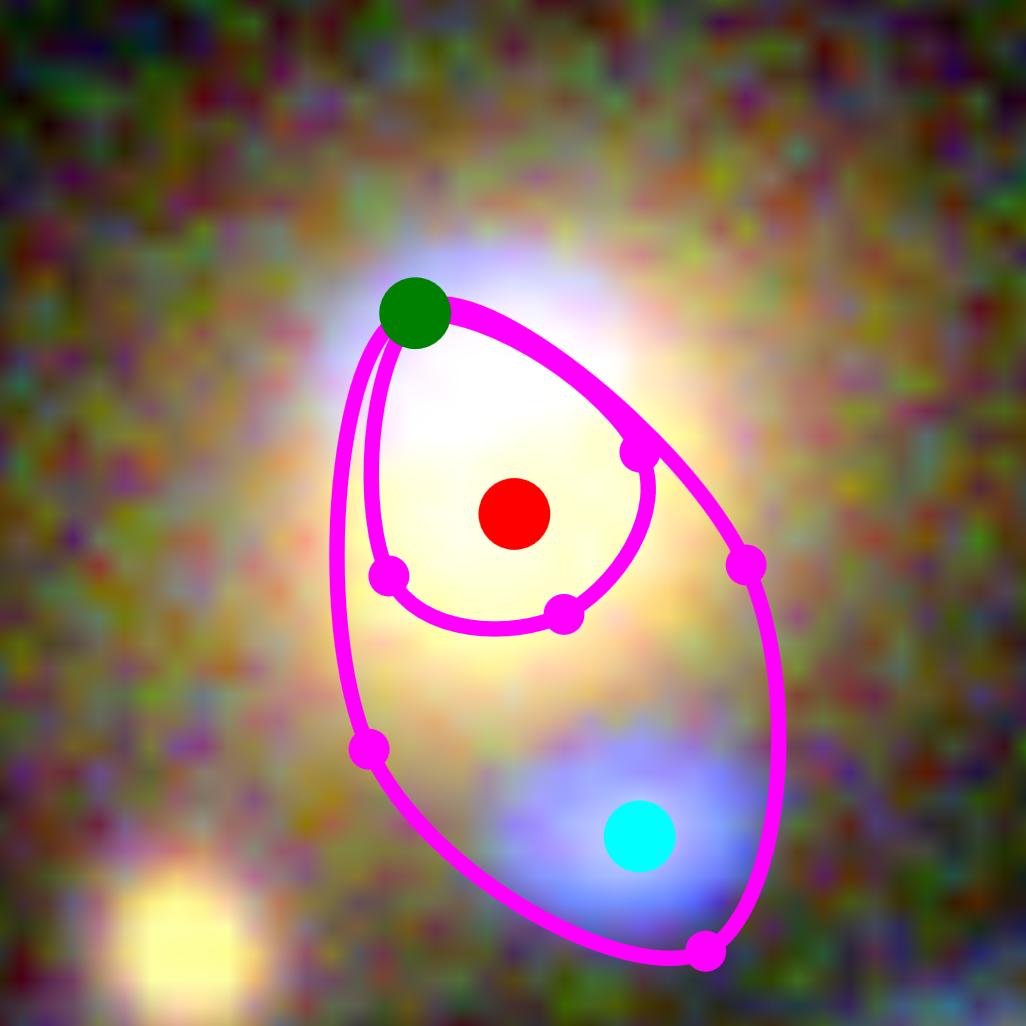
\includegraphics[width=\myplotswidth]{fig/006937_input}
  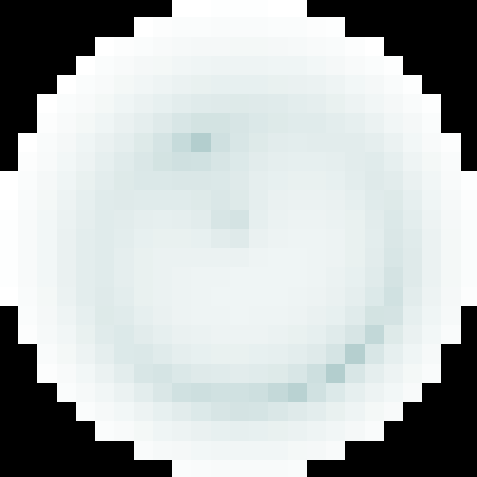
\includegraphics[width=\myplotswidth]{fig/006937_arr_time} \\
  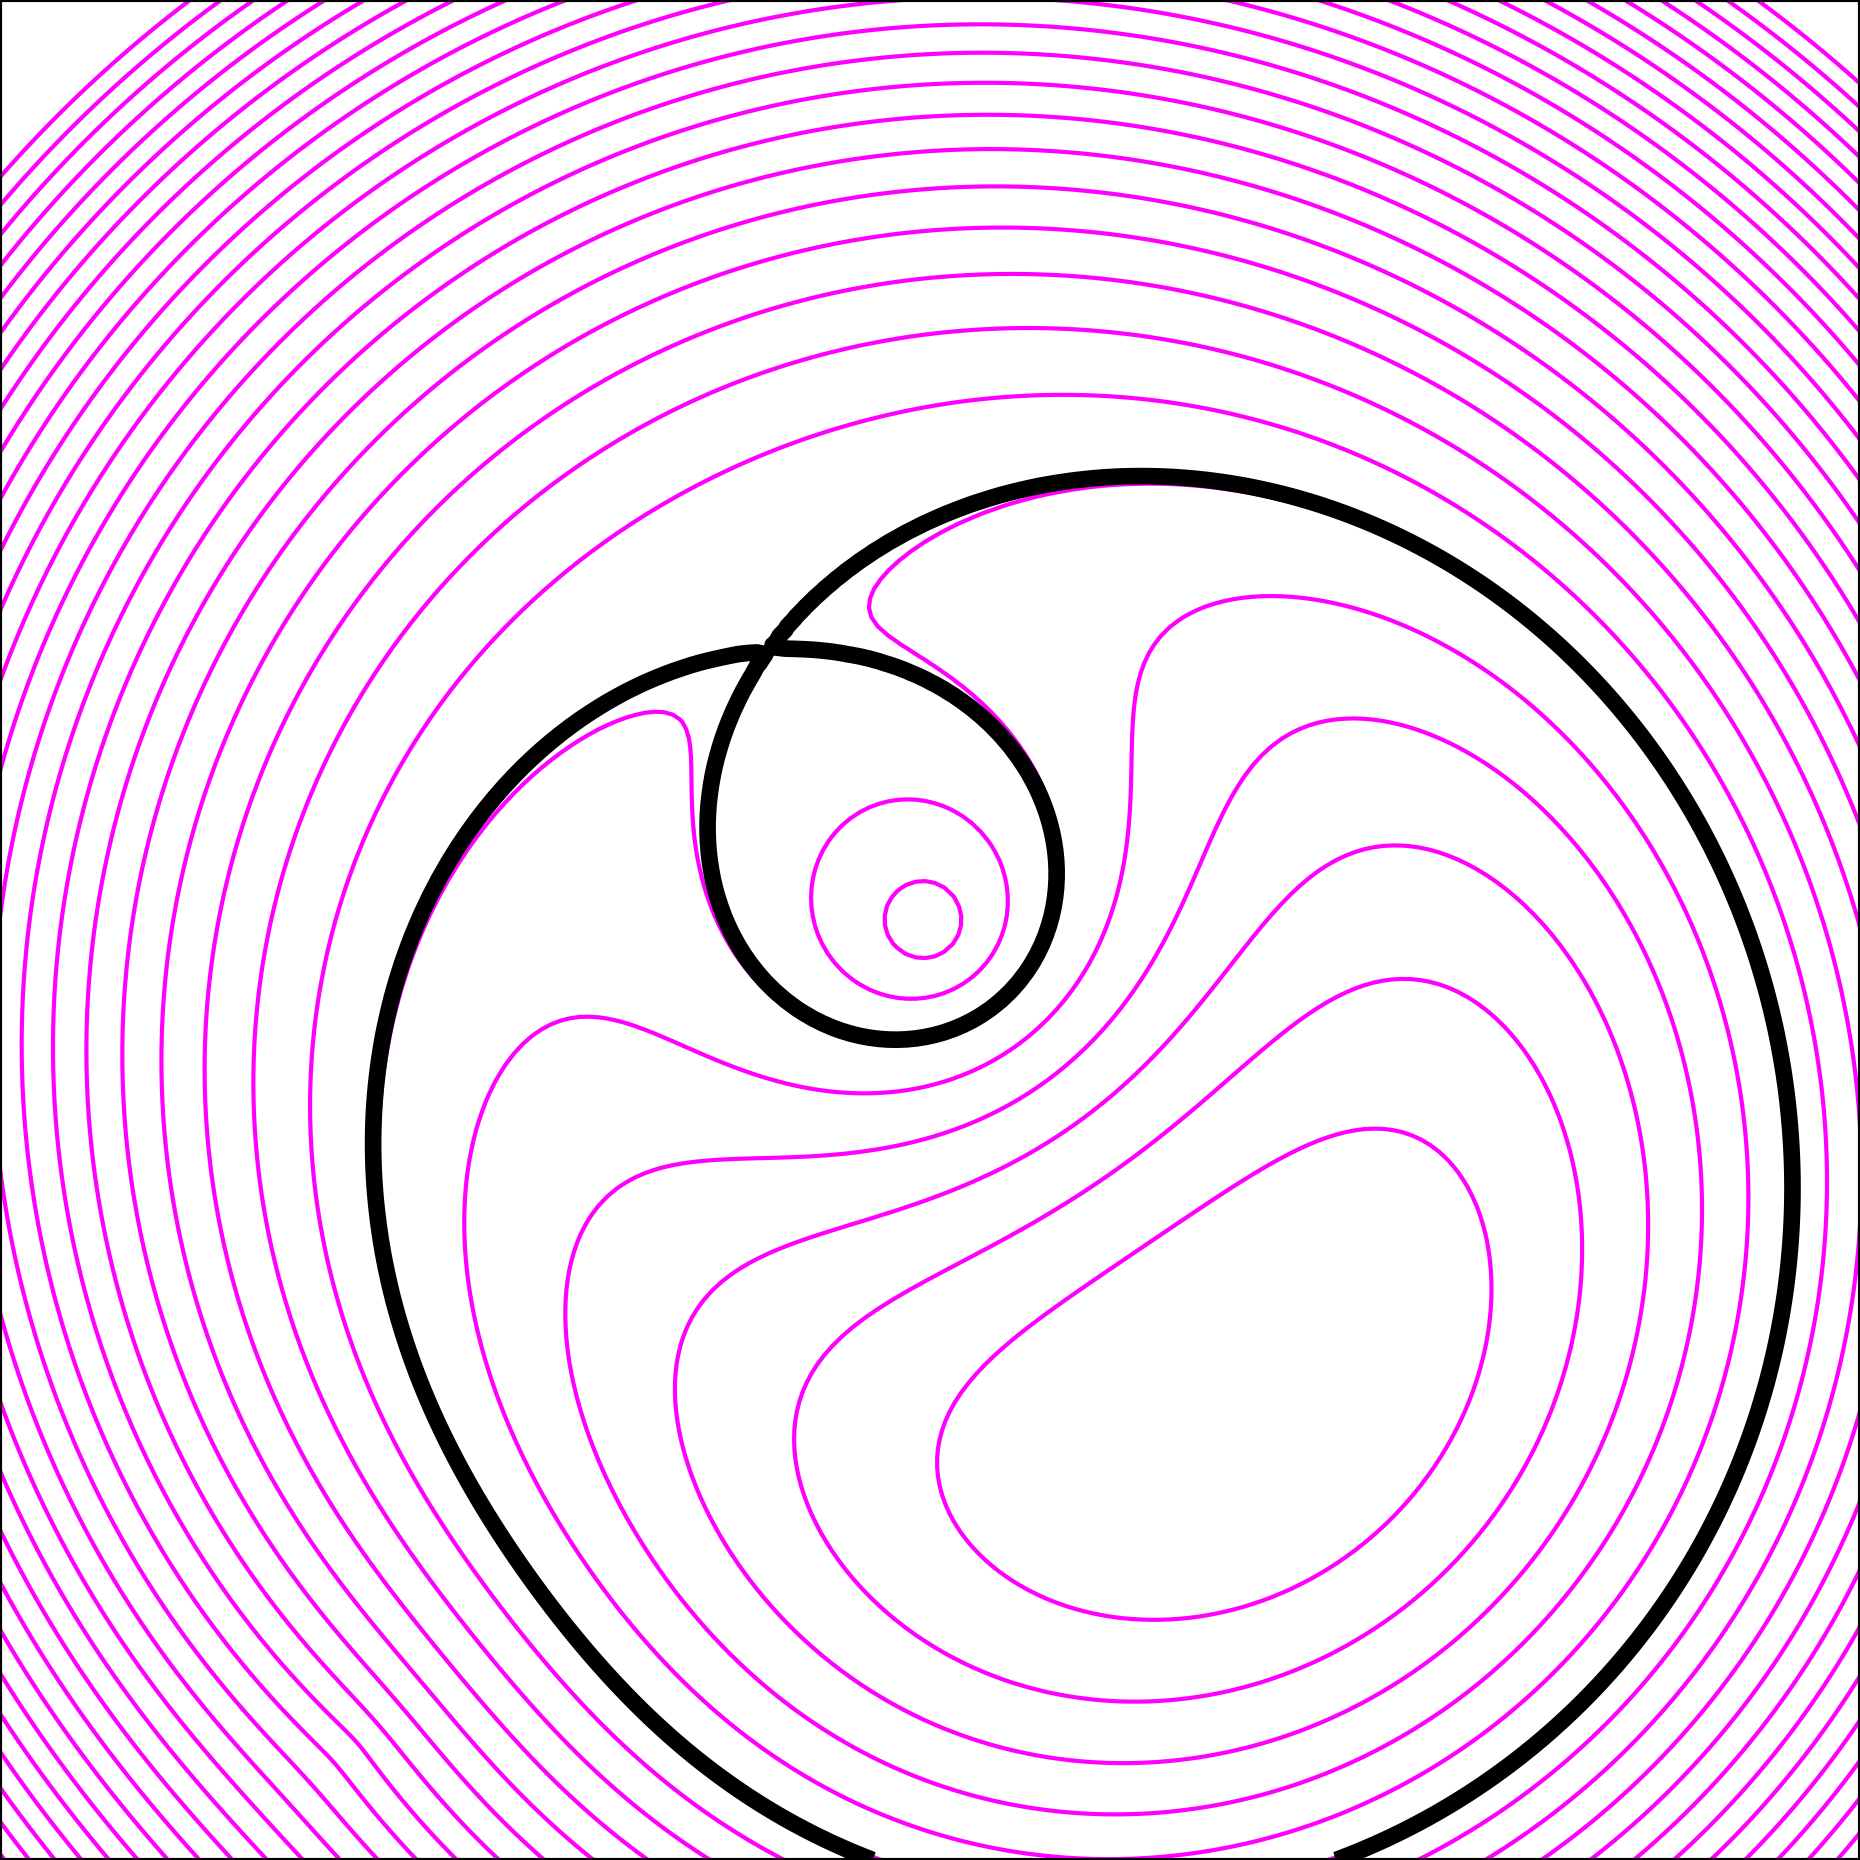
\includegraphics[width=\myplotswidth]{fig/ASW0000vqg_006937_arriv}
  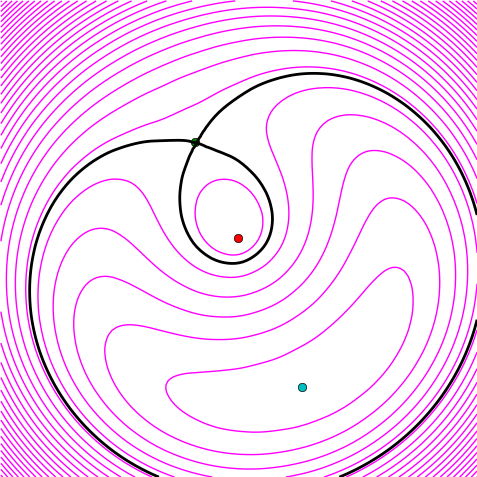
\includegraphics[width=\myplotswidth]{fig/006937_spaghetti} \\
  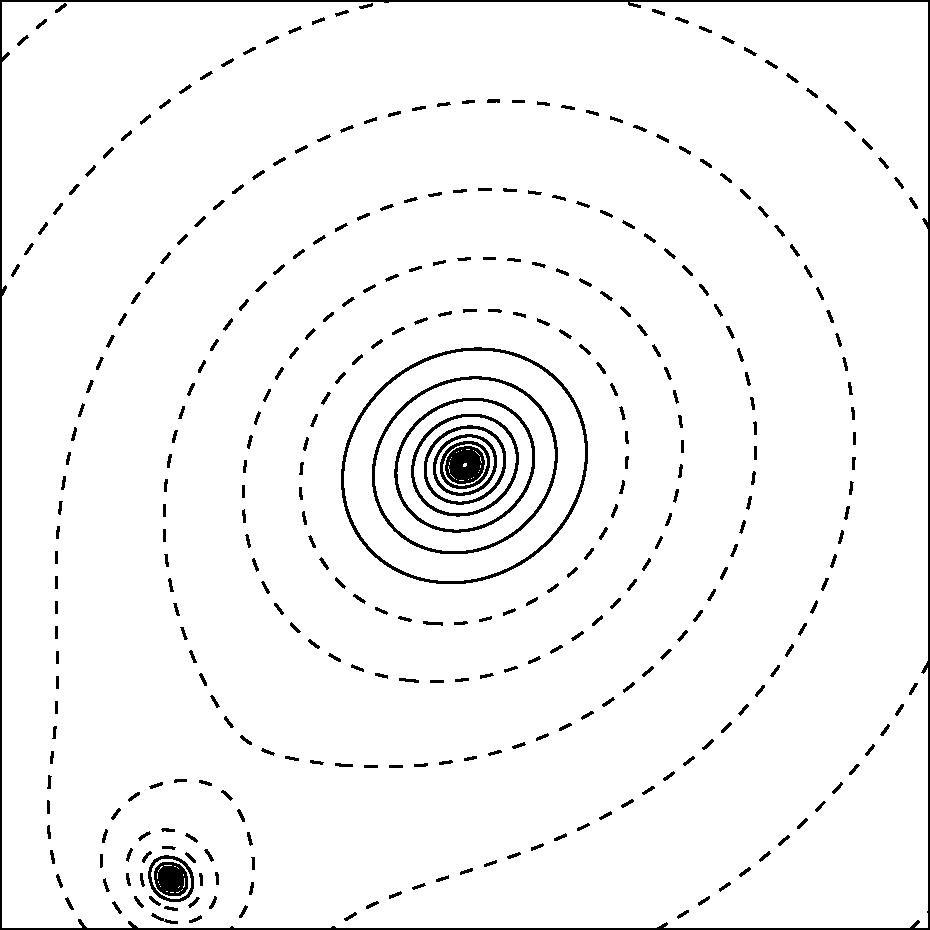
\includegraphics[width=\myplotswidth]{fig/ASW0000vqg_006937_kappa}
  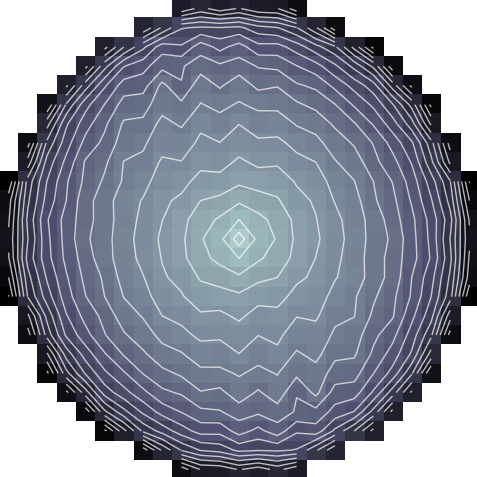
\includegraphics[width=\myplotswidth]{fig/006937_mass}

  \caption[result 6937 (ASW0000vqg)]{A sim with unrecovered
    substructure, resulting in a poor mass model. (See Section
    \ref{sec:example_models} for details.)}
  \label{fig:6937}
\end{figure}

\begin{figure}
  \centering

  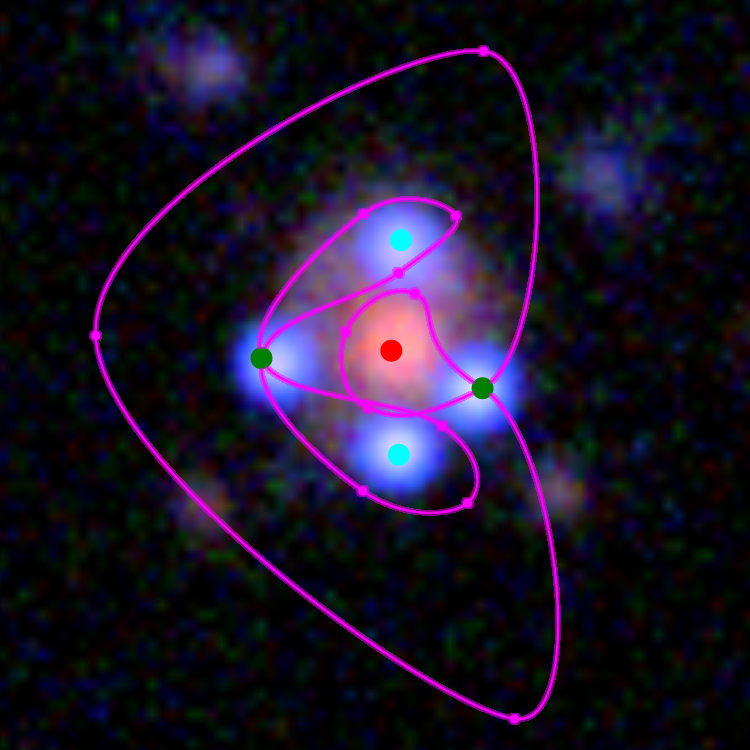
\includegraphics[width=\myplotswidth]{fig/007025_input}
  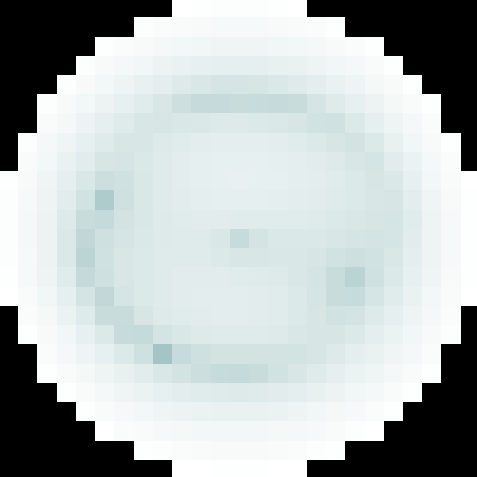
\includegraphics[width=\myplotswidth]{fig/007025_arr_time} \\
  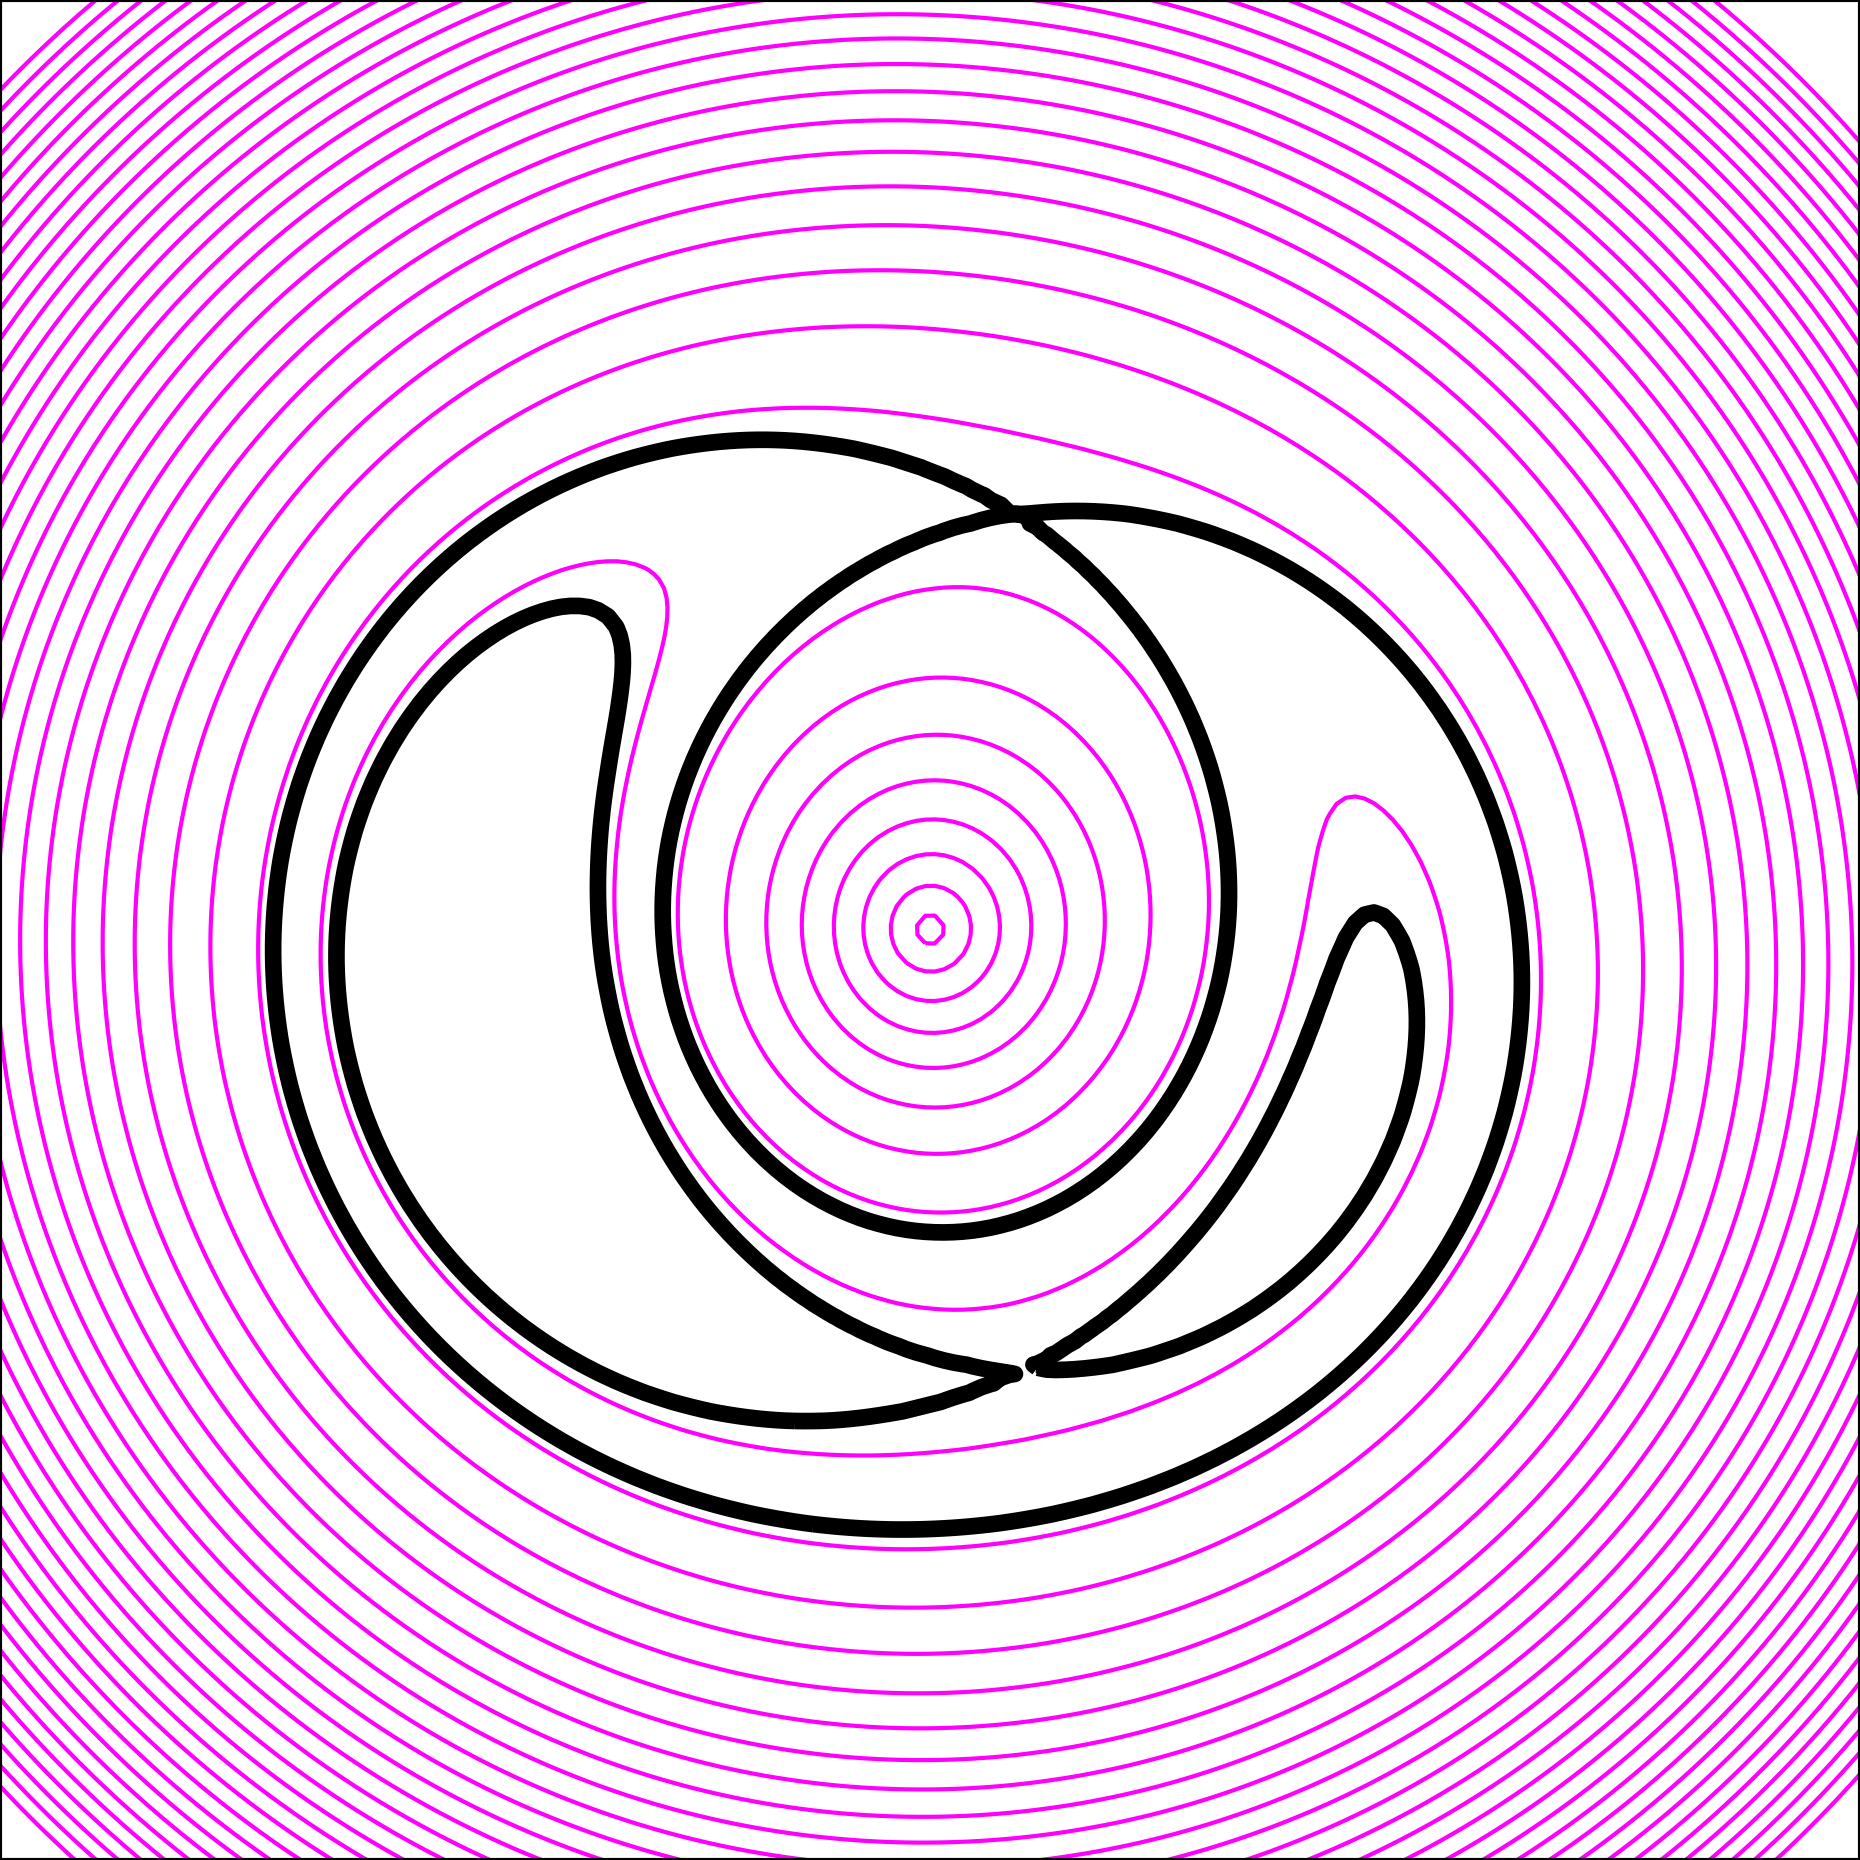
\includegraphics[width=\myplotswidth]{fig/ASW0000h2m_007025_arriv}
  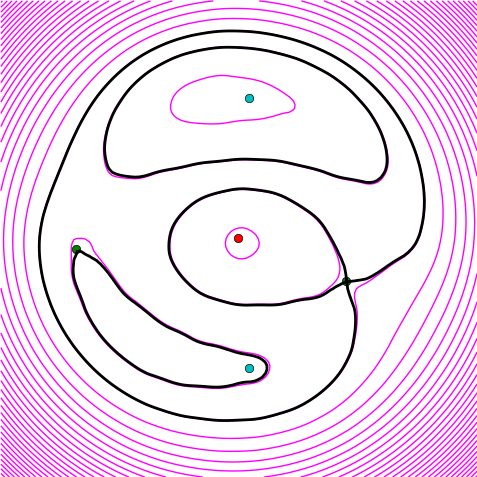
\includegraphics[width=\myplotswidth]{fig/007025_spaghetti} \\
  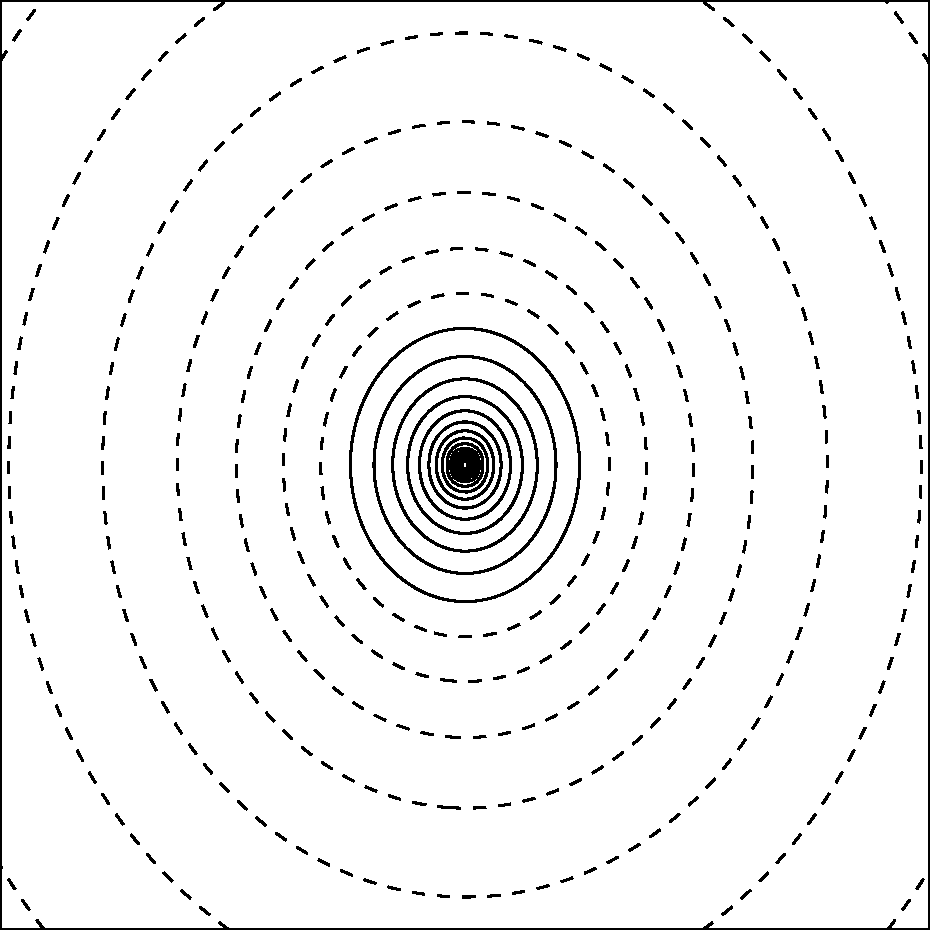
\includegraphics[width=\myplotswidth]{fig/ASW0000h2m_007025_kappa}
  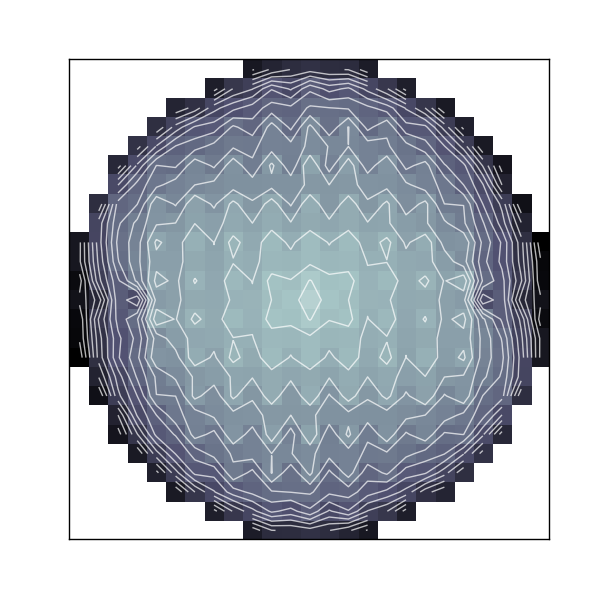
\includegraphics[width=\myplotswidth]{fig/007025_mass}
  \caption[result 7025 (ASW0000h2m)]{A four-image system with image
    parities incorrectly identified.  The model is poor, but the
    estimated Einstein radius is not bad. (See Section
    \ref{sec:example_models} for details.)}
  \label{fig:7025}
\end{figure}

\begin{figure}
  \centering


  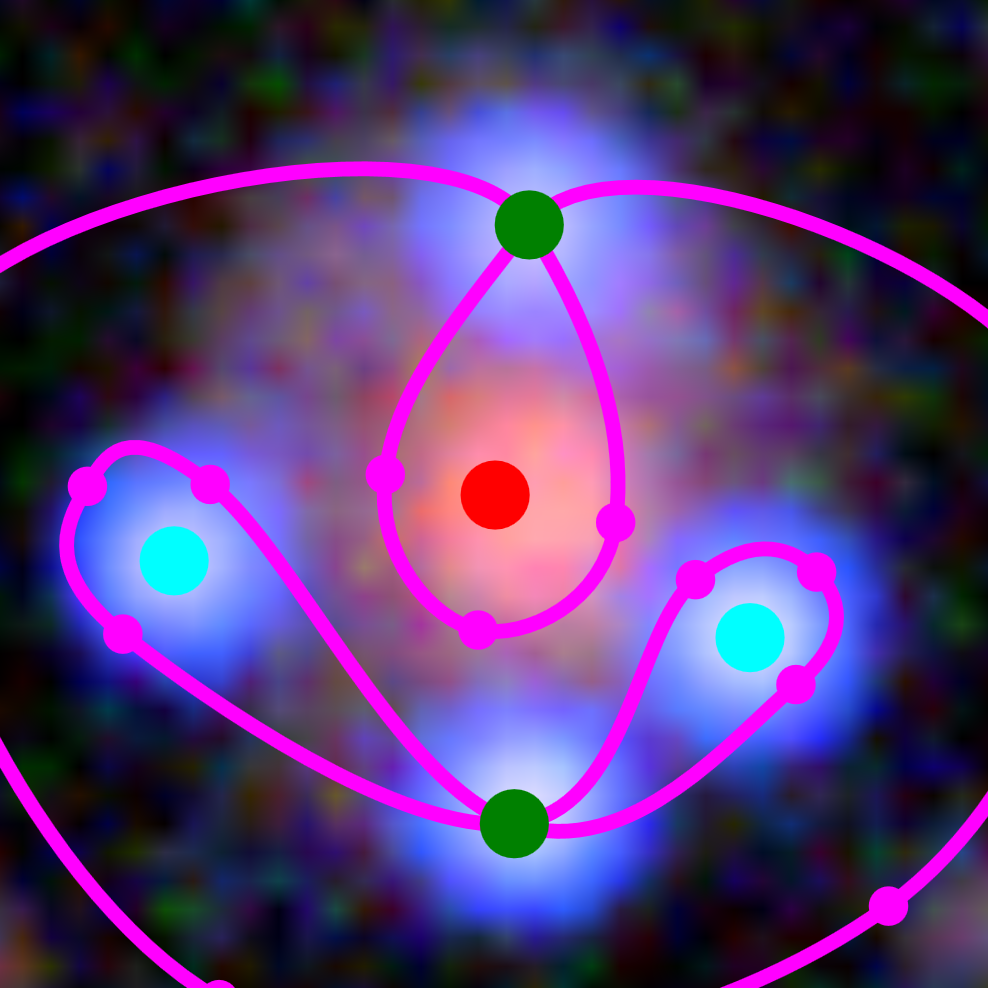
\includegraphics[width=\myplotswidth]{fig/007022_input}
  
\includegraphics[width=\myplotswidth]{fig/007022_arr_time} \\
  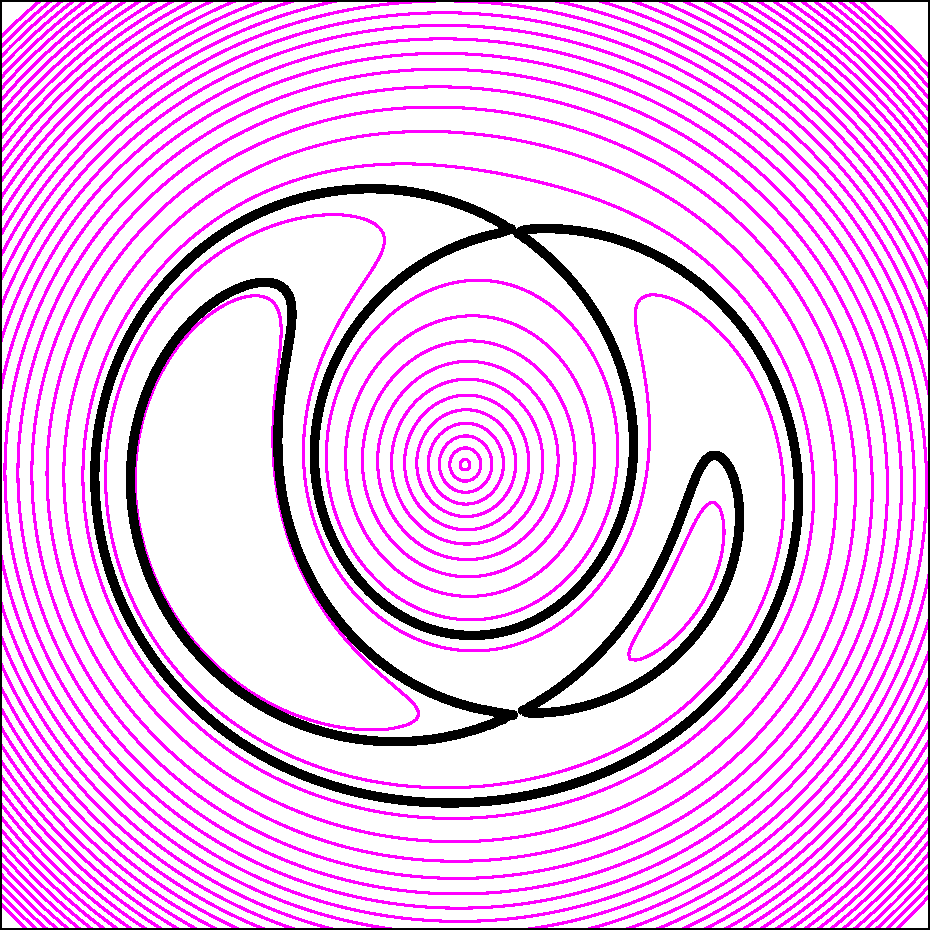
\includegraphics[width=\myplotswidth]{fig/ASW0000h2m_007022_arriv}
  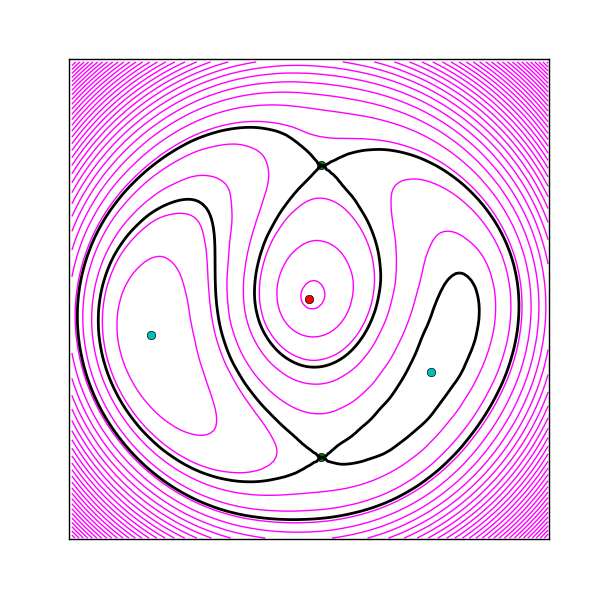
\includegraphics[width=\myplotswidth]{fig/007022_spaghetti} \\
  \includegraphics[width=\myplotswidth]{fig/ASW0000h2m_007022_kappa}
  \includegraphics[width=\myplotswidth]{fig/007022_mass}

  \caption[result 7022 (ASW0000h2m)]{The same system as in Figure
    \ref{fig:7025}, this time with image parities correctly
    identified. (See Section \ref{sec:example_models} for details.)}
  \label{fig:7022}
\end{figure}

\FloatBarrier

Figures \ref{fig:6941}--\ref{fig:7022} show details of eight models.
The first four of these show the most common image morphologies, the
other four explain some problem cases.  Each of the figures has the
following layout.
$$ \begin{matrix}
\hbox{marked-up image} \qquad &\hbox{model synthetic image} \\
t(x,y)                        &\hbox{model } t(x,y) \\
\kappa(x,y)                   &\hbox{model } \kappa(x,y)
\end{matrix} $$
The marked-up image is a zoom of the lensed image on Spacewarps,
marked up with one or more spaghetti contours; this is the modeller's
input to \spl.  The three panels on the right show the graphical
output returned to the modeller by \spl, listed as (i), (ii), (iii) in
\S\ref{sec:SpaghettiLens}).  These derive from the mean of an ensemble
of 200 models generated by \spl.  To generate the synthetic image,
\spl assumes a simple conical source profile.  The user can change the
contrast level on the image, which (though it is not saved) amounts to
adjusting the width of the cone.  These synthetic images are still
very crude and not useful for assessing models.  The best indicator of
whether the modelling was successful is the arrival-time surface
$t(x,y)$, shown as contour maps. Contours passing through saddle
points are shown in black: these are the model versions of the
spaghetti sketch provided by the user.  The model $\kappa(x,y)$ is
shown as a contour map superimposed on an intensity map. A fairly
smooth mass distribution, as here, is a good sign.  An irregular or
checkboard pattern in the mass map usually indicates a bad model.

Figure \ref{fig:6941} shows a simple example.  In summary: the
identification of minimum and saddle point is correct, but the
estimated Einstein radius is a little too high.

Figure \ref{fig:6915} shows another quad.  This kind of configuration
arises when the mass is elongated and the source is displaced at an
angle to the elongation.

Figure \ref{fig:6990} shows an example of an arc that has split into
three images.  This kind of configuration, with a counter-image close
to the lensing galaxy and a more distant arc/triplet on the other
side, generically arises from an elongated mass distribution when the
source is displaced along the elongated direction.

To conclude this set of examples, Figure \ref{fig:6919} shows another
type of quad.  Actually, in this case the brightest part of the source
is only doubly imaged, but the source extends into a region that
produces four images.  We can also see from the real arrival-time
surface that a point source is a double on the verge of splitting into
a quad.  The modeler interpreted the system as a quad.  The
appearance of the arcs, shown in the bottom panel of Figure
\ref{fig:input-spag}, looks like an arc and counter-image such as
discussed with Figure \ref{fig:6990} above.  But there is an important
difference: the long arc is closer to the galaxy, as if the arc and
counter-image have swapped roles.  This configuration arises if the
source displacement is perpendicular to the long axis of the lensing
mass.


Figure \ref{fig:6975} shows a lens with substructure in the form of a
smaller secondary galaxy.  The galaxies in such group or cluster sims
were, in fact, based on galaxies visible in the images --- but the
modelers were not told in advance whether this was the case.  The
model does not include any substructure, but otherwise is not bad.
The minimum and saddle point are correct, and the Einstein radius is
only a little underestimated.

Figure \ref{fig:6937} shows a case where substructure leads to a
poor model.


Figure \ref{fig:7022} shows another model of the same system.  In this
one, the identification of the minima and saddle points was incorrect,
and mass distribution comes out elongated East-West instead of
North-South.  The mass distribution also appears somewhat jagged and
the saddle-point contours are not as clean as in the previous
examples; these are often indicators of a problem with the model.  The
enclosed mass is, however, none the worse --- the reason is probably
that in a relatively symmetrical image configuration, the Einstein
radius is quite well constrained by the images in a fairly
model-independent way.


Figure \ref{fig:6975} shows a fairly symmetric quad.  The minima and
saddle points are correctly identified, and the orientation of the
ellipticity of the mass distribution is correctly reproduced.  The
Einstein radius is somewhat overestimated.  

Figure \ref{fig:kapenc_compare_faulty} shows a comparison of input and
recovered mass profiles.  The panel shows a average $\kappa$ within a
given radius, as a function of radius.  The red curve is the true
value, and where it crosses unity (dotted horizontal line) is the
notional Einstein radius $\Theta_{\text{E, sim}}$.  The two blue
curves are the minimal and maximal mean enclosed $\kappa$ from the
internal ensemble in \spl.  The region between the blue curves is
shaded between the radii of the innermost and the outermost images ---
this is the confidence region from the modeling.  As we see, the
shaded blue is slightly above the red curve.  The Einstein Radius
$\Theta_\text{E}$ of the model is estimated crossing the mean enclosed
$\kappa$ (not plotted) with unity.


The panel shows
a average $\kappa$ within a given radius, as a function of radius.
The red curve is the true value, and where it crosses unity (dotted
horizontal line) is the notional Einstein radius $\Theta_{\text{E, sim}}$.
  The two blue curves
are the minimal and maximal mean enclosed $\kappa$ from the internal
ensemble in \spl.  The region between the blue curves is shaded
between the radii of the innermost and the outermost images --- this
is the confidence region from the modeling.  As we see, the shaded
blue is slightly above the red curve. 
The Einstein Radius $\Theta_\text{E}$ of the model is estimated crossing the
mean enclosed $\kappa$ (not plotted) with unity.
